%%%%%%%%%%%%%%%%%%%%%%%%%%%%%%%%%%%%%%%%%%%%%%%%%%%%%%
% A Beamer template for University of Wollongong     %
% Based on THU beamer theme                          %
% Author: Qiuyu Lu                                   %
% Date: July 2024                                    %
% LPPL Licensed.                                     %
%%%%%%%%%%%%%%%%%%%%%%%%%%%%%%%%%%%%%%%%%%%%%%%%%%%%%%
% Customized for Sharif University of Technology     %
%%%%%%%%%%%%%%%%%%%%%%%%%%%%%%%%%%%%%%%%%%%%%%%%%%%%%%


\documentclass[serif, aspectratio=169]{beamer}
%\documentclass[serif]{beamer}  % for 4:3 ratio
\usepackage[T1]{fontenc} 
\usepackage{fourier} % see "http://faq.ktug.org/wiki/uploads/MathFonts.pdf" for other options
\usepackage{hyperref}
\usepackage{latexsym,amsmath,xcolor,multicol,booktabs,calligra}
\usepackage{graphicx,pstricks,listings,stackengine}
\usepackage{lipsum}
\usepackage{algorithm, algpseudocode, mathtools, needspace}
\usepackage{tikz}



\author{Ali Sharifi-Zarchi}
\title{Machine Learning (CE 40717)}
\subtitle{Fall 2024}
\institute{
    CE Department \\
    Sharif University of Technology
}
%\date{\small \today}
% \usepackage{UoWstyle}
\usepackage{SUTstyle}

% defs
\def\cmd#1{\texttt{\color{red}\footnotesize $\backslash$#1}}
\def\env#1{\texttt{\color{blue}\footnotesize #1}}
\definecolor{deepblue}{rgb}{0,0,0.5}
\definecolor{deepred}{RGB}{153,0,0}
\definecolor{deepgreen}{rgb}{0,0.5,0}
\definecolor{halfgray}{gray}{0.55}
\DeclareMathOperator*{\argmax}{argmax}
\DeclareMathOperator*{\argmin}{argmin}

\lstset{
    basicstyle=\ttfamily\small,
    keywordstyle=\bfseries\color{deepblue},
    emphstyle=\ttfamily\color{deepred},    % Custom highlighting style
    stringstyle=\color{deepgreen},
    numbers=left,
    numberstyle=\small\color{halfgray},
    rulesepcolor=\color{red!20!green!20!blue!20},
    frame=shadowbox,
}


\begin{document}

\begin{frame}
    \titlepage
    \vspace*{-0.6cm}
    \begin{figure}[htpb]
        \begin{center}
            
\includegraphics[keepaspectratio, scale=0.25]{pic/sharif-main-logo.png}
        \end{center}
    \end{figure}
\end{frame}

\begin{frame}    
\tableofcontents[sectionstyle=show,
subsectionstyle=show/shaded/hide,
subsubsectionstyle=show/shaded/hide]
\end{frame}

\section{Introduction}

\begin{frame}{High Dimensional Data}
    \begin{itemize}
        \item High dimensions has many features.
        \item EEG signals from the brain, recorded with 56 channels and 3000 time points per trial.

        \begin{figure}[htpb]
            \begin{center}
                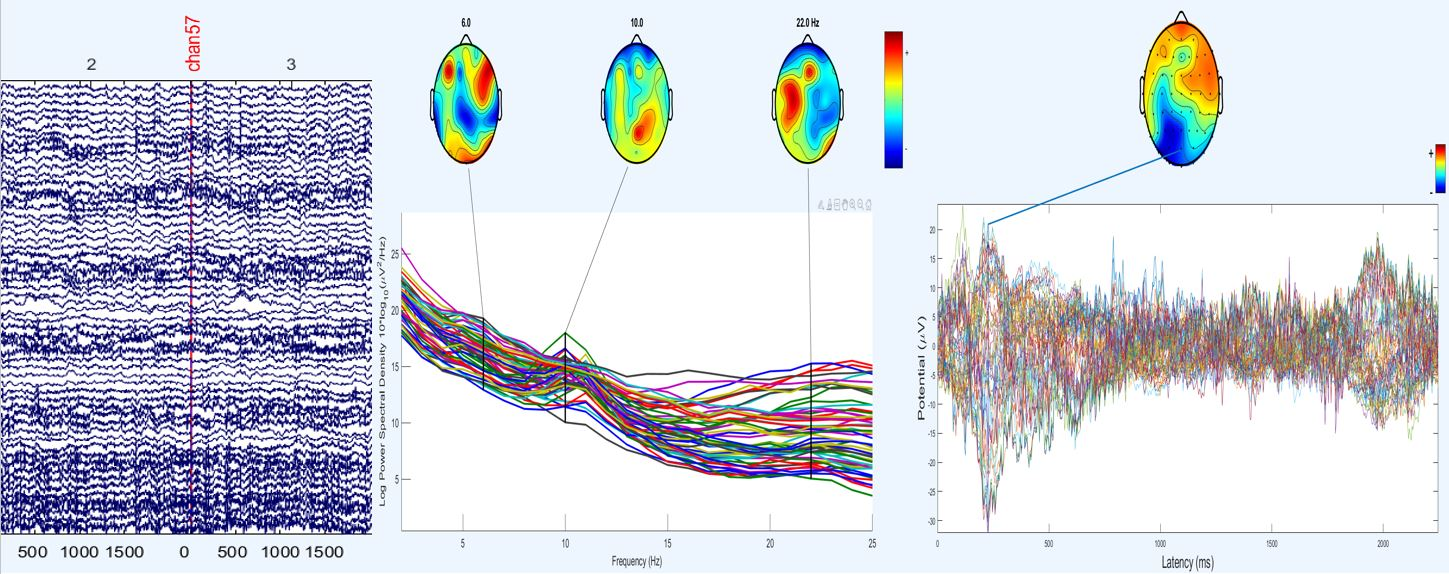
\includegraphics[keepaspectratio, scale=0.4]{pic/brain.JPG}
            \end{center}
        \end{figure}
    \end{itemize}
\end{frame}

\begin{frame}{High Dimensional Data}
    \begin{itemize}
        \item Social media
        \hspace{0.5}
        \begin{figure}[htpb]
            \begin{center}
      
\includegraphics[keepaspectratio, scale=0.4]{pic/social.png}
             \caption{\href{https://redeemedlifecounseling.com/why-we-share-everything-on-social-media/}{Figure reference}}
            \end{center}
        \end{figure}
    \end{itemize}
\end{frame}

\begin{frame}{High Dimensional Data}
    \begin{itemize}
        \item Customer purchase data
        \begin{figure}[htpb]
            \begin{center}
                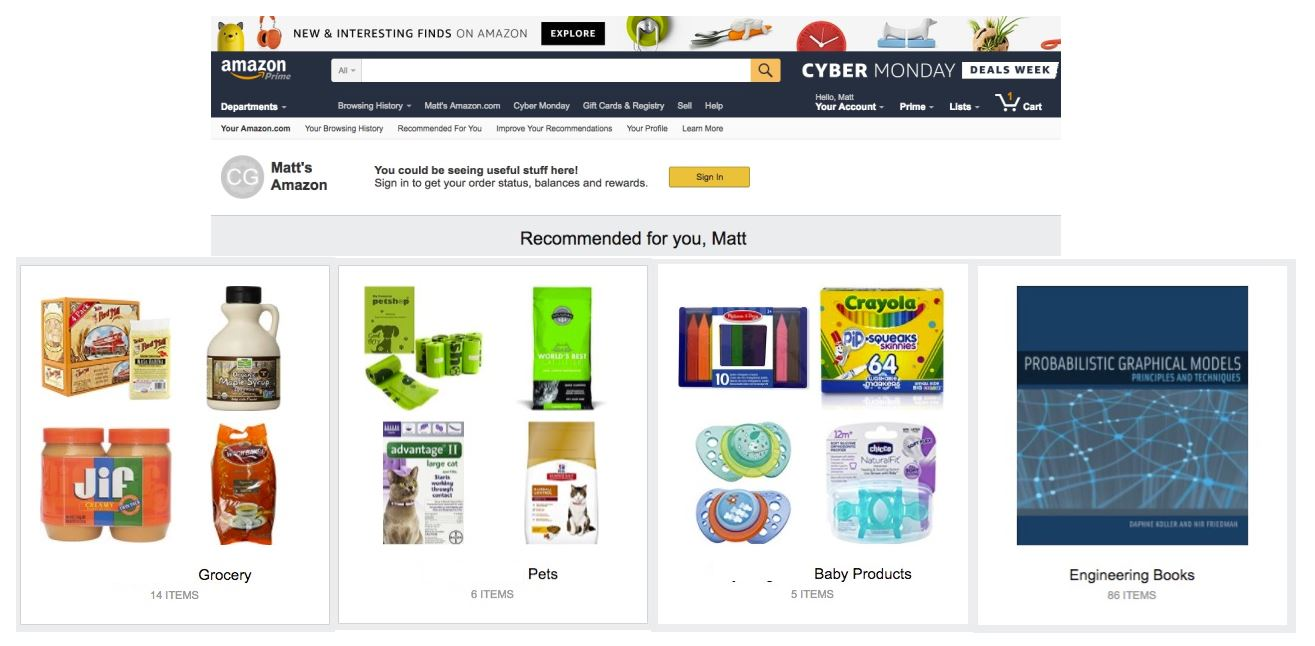
\includegraphics[keepaspectratio, scale=0.4]{pic/customer_data.JPG}
            \end{center}
        \end{figure}
    \end{itemize}
\end{frame}


\begin{frame}{Dimensionality Reduction Benefits}
    \begin{itemize}
        \item \textbf{Visualization}
            \begin{itemize}
                \item Project high dimensional data into 2D or 3D.
            \end{itemize}
        \item \textbf{Helps avoid overfitting}
            \begin{itemize}
                \item Reducing noise by reducing features.
                \item Improves accuracy by reducing noise.
            \end{itemize}
        \item \textbf{More efficient use of resources}
            \begin{itemize}
                \item Time, Memory, CPU
            \end{itemize}
    \end{itemize}
\end{frame}

\begin{frame}{Dimensionality Reduction Techniques}
    \begin{itemize}
        \item \textbf{Feature Selection}
            \begin{itemize}
                \item Select a subset from a given feature set.
            \end{itemize}

         \item \textbf{Feature Extraction}
            \begin{itemize}
                \item A linear or non-linear transform from the original feature space to a lower dimension space.
            \end{itemize}
            \begin{figure}[htpb]
                \begin{center}
                    \includegraphics[keepaspectratio, scale=0.20]{pic/FS-FE.png}
                    \caption{\href{https://link.springer.com/article/10.1007/s00500-019-04628-6}{Figure reference}}
                \end{center}
            \end{figure}
    \end{itemize}
\end{frame}

\begin{frame}{Dimensionality Reduction Purpose}
    \begin{itemize}
        \item Maximize retention of  \textbf{important information} while reducing dimensionality.
        
        \item What is \textbf{important information}?
    \end{itemize}
\end{frame}

\begin{frame}{Purpose: Variance of Data}
    \begin{itemize}
        \item Maximize retention of  \textbf{important information} while reducing dimensionality.
        \item \textbf{Information:} Variance of projected data
        \begin{figure}[htpb]
                \begin{center}
                    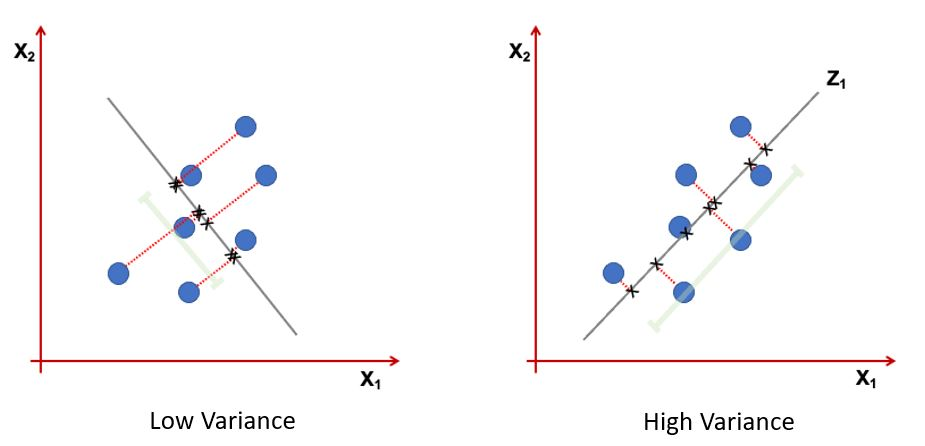
\includegraphics[keepaspectratio, scale=0.5]{pic/dim_red_var.JPG}
                    \caption{\href{https://bookdown.org/tpinto_home/Unsupervised-learning/principal-components-analysis.html}{Figure reference}}
                \end{center}
        \end{figure}
    \end{itemize}

\end{frame}

\begin{frame}{Purpose: Local Geometric Neighborhood}
    \begin{itemize}
        \item \textbf{Information:} Preserve local geometric neighborhood.
        \begin{figure}[htpb]
                \begin{center}
                    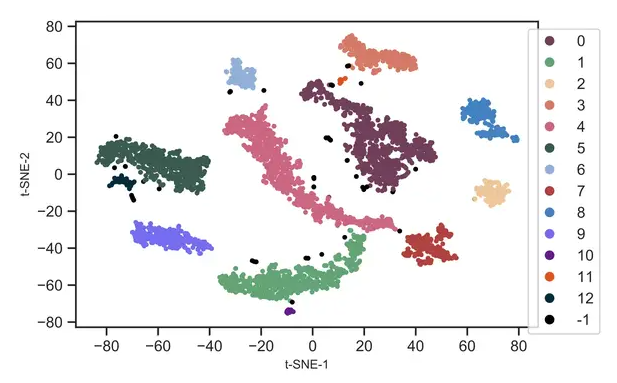
\includegraphics[keepaspectratio, scale=0.5]{pic/local_relation.PNG}
                  \caption{\href{https://www.reneshbedre.com/blog/tsne.html}{Figure reference}}
                \end{center}
        \end{figure}
    \end{itemize}
\end{frame}

\begin{frame}{Purpose: Local and Global Geometric Neighborhood}
    \begin{itemize}
        \item \textbf{Information:} Preserve both local and global geometric neighborhood.
        \begin{figure}[htpb]
                \begin{center}
                    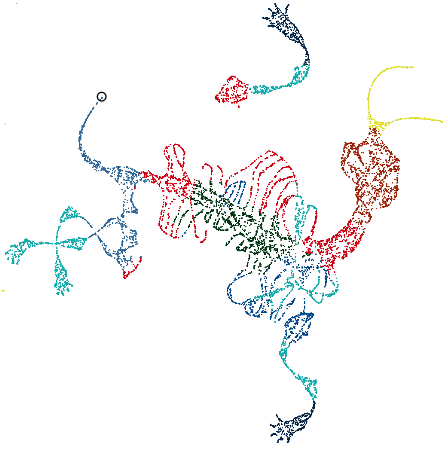
\includegraphics[keepaspectratio, scale=0.45]{pic/global_relation.PNG}
                  \caption{\href{https://pair-code.github.io/understanding-umap/#:~:text=The}{Figure reference}}
                \end{center}
        \end{figure}
    \end{itemize}
\end{frame}

% \begin{frame}{Purpose: Statistical Independence}
%     \begin{itemize}
%         \item Maximize retention of  \textbf{important information} while reducing dimensionality
%         \item \textbf{Information:} Statistical independence of projections directions
%         \begin{figure}[htpb]
%                 \begin{center}
%                     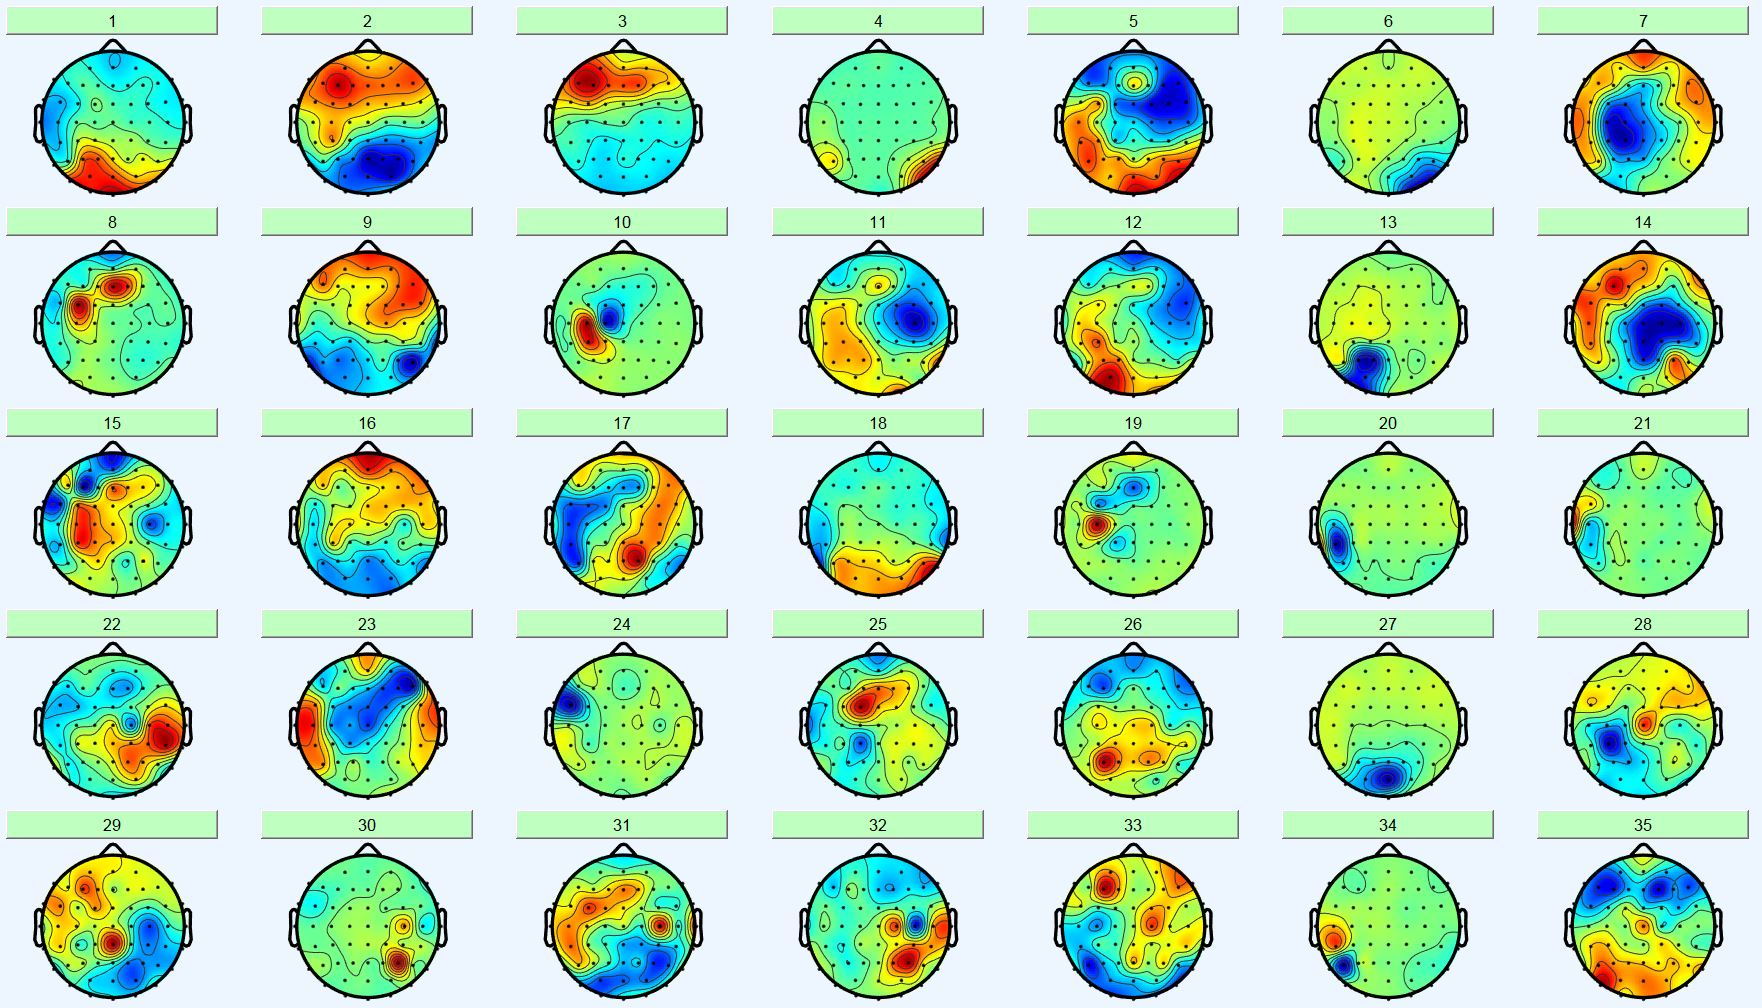
\includegraphics[keepaspectratio, scale=0.25]{pic/dim_red_independent.JPG}
%                 \end{center}
%         \end{figure}
%     \end{itemize}
% \end{frame}

\section{Principal Component Analysis (PCA)}

\begin{frame}{Idea}
    \begin{itemize}
        \item Given data points in a d-dimensional space, project them into a lower dimensional space while preserving as much information as possible:
        \begin{itemize}
            \item Find the best planar approximation of 3D data.
            \item Find the best 12-D approximation of 104-D data.
        \end{itemize}
        \item In particular, choose projection that minimizes the squared error in reconstructing the original data.
    \end{itemize}
\end{frame}

\begin{frame}{Principal Components Idea}
    \begin{itemize}
        \item 2D Gaussian dataset:
         \begin{figure}[htpb]
            \begin{center}
                \includegraphics[keepaspectratio, scale=0.6]{pic/pcaData.JPG}
            \end{center}
        \end{figure}
    \end{itemize}
\end{frame}

\begin{frame}{Principal Components Idea}
    \begin{itemize}
        \item First PCA axis:
         \begin{figure}[htpb]
            \begin{center}
                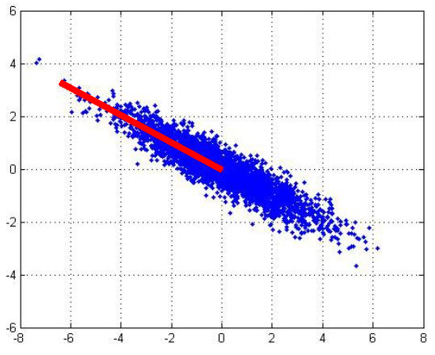
\includegraphics[keepaspectratio, scale=1]{pic/pcaData1.JPG}
            \end{center}
        \end{figure}
    \end{itemize}
\end{frame}

\begin{frame}{Principal Components Idea}
    \begin{itemize}
        \item First and second PCA axes:
         \begin{figure}[htpb]
            \begin{center}
                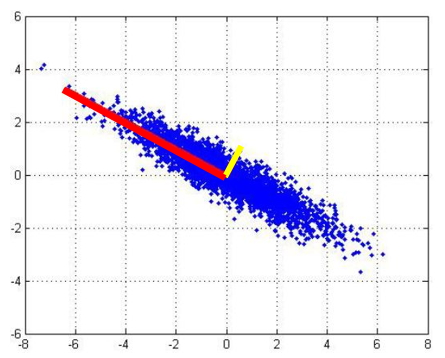
\includegraphics[keepaspectratio, scale=1]{pic/pcaData2.JPG}
            \end{center}
        \end{figure}
    \end{itemize}
\end{frame}

\begin{frame}{Random vs. Principal Projection}
    \begin{itemize}
        \item Random direction versus principal component:
        \begin{figure}[htpb]
            \begin{center}
                \includegraphics[keepaspectratio, scale=0.8]{pic/pcaVSrandom.JPG}
            \end{center}
        \end{figure}
    \end{itemize}
\end{frame}


\begin{frame}{Definition}
    \begin{itemize}
        \item \textbf{Goal}: reducing the dimensionality of the data while preserving important aspects of the data.
        \item Suppose $\mathbf{X} = \begin{pmatrix} \mathbf{X}_1^T \\ \vdots \\ \mathbf{X}_N^T \end{pmatrix}_{N \times d} = \begin{pmatrix}  
\overset{\displaystyle F_1}x_{11} & \overset{\displaystyle F_2}x_{12} & \hdots & \overset{\displaystyle F_d}x_{1d} \\
x_{21} & x_{22} & \hdots & x_{2d} \\
\vdots \\
x_{N1} & x_{N2} & \hdots & x_{Nd} \\
\end{pmatrix} $
        \item $\mathbf{X}_{N \times d} \xrightarrow{\text{PCA}} \tilde{\mathbf{X}}_{N \times k} \quad \text{with} \quad k \leq d$
        \item \textbf{Assumption}: Data is mean-centered, which is: $\mu_x = \frac{1}{N} \sum_{i=1}^{N}X_i = 0_{d \times 1}$
    \end{itemize}
\end{frame}

\begin{frame}{Interpretations}
    Orthogonal projection of the data onto a \textbf{lower-dimensional} linear \textbf{subspace} that:
    \begin{itemize}
        \item \textbf{Interpretation 1.} Maximizes variance of projected data.
        \item \textbf{Interpretation 2.} Minimizes the sum of squared distances to the subspace.
    \end{itemize}
    \begin{figure}[htpb]
        \begin{center}
            \includegraphics[keepaspectratio, scale=0.4]{pic/pca.png}
        \end{center}
    \end{figure}
\end{frame}

\begin{frame}{Equivalence of the Interpretations}
    \begin{itemize}
        \item Minimizing the sum of square distances to the subspace is \textbf{equivalent} to maximizing the sum of squares of the projections on that subspace.
    \end{itemize}
    \begin{figure}[htpb]
        \begin{center}
            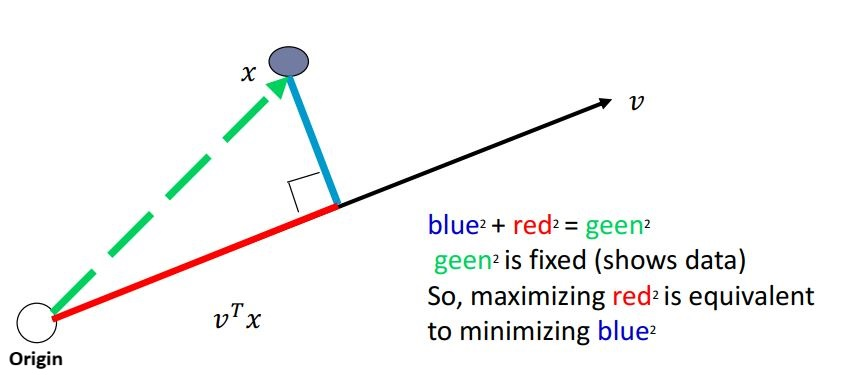
\includegraphics[keepaspectratio, scale=0.55]{pic/var_vs_rec2.JPG}
        \end{center}
    \end{figure}
\end{frame}

% \begin{frame}{Equivalence of the Interpretations}

%     \textbf{Principal Components (PCs)}: A set of \textbf{orthonormal} vectors $(\nu = [\nu_1, \nu_2, ...,\nu_k])$ (where each $\nu_i$ is $d\times 1$) generated by PCA, which fulfill both of the interpretations.\\[0.4cm]
    
%     Interpretation 1. Maximizes variance of projected data\\[0.3cm]
%     \begin{itemize}
%         \item Projection of data points on $\nu_1$
%         $$\Pi = \Pi_{\nu_1} \{ X_{1}, \dots, X_{N} \} = \{ \nu_1^T X_{1}, \dots, \nu_1^T X_{N} \}$$
%         \item Note that $\text{Var}(X) = \mathbb{E}[X^2] - \mathbb{E}[X]^2$
%         $$\mathbb{E}[X] = 0 \rightarrow \text{Var}(\Pi) = \frac{1}{N} \left( \sum_{i=1}^{N} (\nu_1^T X_i)^2 \right)$$
%     \end{itemize}
    
% \end{frame}

% \begin{frame}{Equivalence of the  Interpretations}
%     Interpretation 1. Maximizes variance of projected data\\[0.3cm]
%     \begin{itemize}
%         \item Based on the assumption, $\frac{1}{N} \sum_{i=1}^{N} X_i = 0$
%         $$\nu^T(\frac{1}{N} \sum_{i=1}^{N} X_i) = 0 \quad \longrightarrow \quad \frac{1}{N} \sum_{i=1}^{N} \nu_1^T X_i = 0$$
%         \item So,
%         $$\text{Var}(\Pi) = \frac{1}{N} \sum_{i=1}^{N} (\nu_1^T X_i)^2$$
%         \item To find $\nu_1$ that maximizes the variance
%         $$\begin{aligned}
%             \argmax_{\nu_1} \quad & \frac{1}{N} \sum_{i=1}^{N} (\nu_1^T X_i)^2\\
%             \textrm{s.t.} \quad & \nu_1^T\nu_1 = 1\\
%         \end{aligned}$$
%     \end{itemize}
% \end{frame}

% \begin{frame}{Equivalence of the Interpretations}
%     Interpretation 2. Minimizes the sum of squared distances to the line\\[0.3cm]
%     \minipage{0.54\textwidth}
%     \begin{itemize}
%         \item Squared distance of one point to the line $$\left\| X_i - (\nu_1^{T}X_i) \nu_1 \right\|_2^2 \quad \text{which } \nu_1^TX_i \text{ is scalar.}$$
%         \item Sum of squared distances $$L_1 = \frac{1}{N} \sum_{i=1}^{N} \left\| X_i - (\nu_1^{T}X_i) \nu_1 \right\|_2^2$$
%     \end{itemize}
%     \endminipage
%     \hfill
%     \minipage{0.42\linewidth}
%     \begin{figure}[htpb]
%             \begin{center}
%                 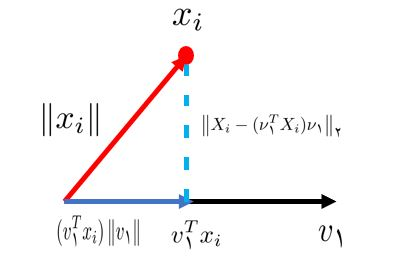
\includegraphics[keepaspectratio, scale=0.7]{pic/varpic.jpg}
%             \end{center}
%         \end{figure}
%     \endminipage
%     \vspace{0.1cm}
%     \begin{itemize}
%         \item By Pythagorean theorem $$L_1 = \frac{1}{N} \sum_{i=1}^{N} (\left\| X_i \right\|^2 - (\nu_1^{T}X_i)^2 \left\|\nu_1 \right\|_2^2) = \underbrace{\frac{1}{N} \sum_{i=1}^{N} (\left\| X_i \right\|^2)}_{\text{constant}} - \frac{1}{N} \sum_{i=1}^{N} ((\nu_1^{T}X_i)^2 \left\|\nu_1 \right\|_2^2) $$
%     \end{itemize}
% \end{frame}

% \begin{frame}{Equivalence of the Interpretations}
%     \textcolor{gray}{Interpretation 2.} Minimizes the sum of squared distances to the line\\[0.2cm]
%     \begin{itemize}
%         \item Removing constant to minimize
%         \item Based on orthonormality, $||V_1||_2^2 = 1$
%         \item To find $\nu_1$ that minimizes the sum of squared distances
%     \end{itemize}
%     \vspace{0.2cm}
%     \minipage{0.45\textwidth}
%     $$\begin{aligned}
%             \argmin_{\nu_1} \quad & -\frac{1}{N} \sum_{i=1}^{N} (\nu_1^T X_i)^2\\
%             \textrm{s.t.} \quad & \nu_1^T\nu_1 = 1\\
%         \end{aligned}$$
%     \endminipage
%     \hfill
%     \minipage{0.1\textwidth}
%     $$\equiv$$
%     \endminipage
%     \hfill
%     \minipage{0.45\linewidth}
%     $$\begin{aligned}
%             \argmax_{\nu_1} \quad & \frac{1}{N} \sum_{i=1}^{N} (\nu_1^T X_i)^2\\
%             \textrm{s.t.} \quad & \nu_1^T\nu_1 = 1\\
%         \end{aligned}$$
%     \endminipage
%     \vspace{0.5cm}
%     \begin{itemize}
%         \item So, the two \textcolor{gray}{interpretations} are equivalent.
%     \end{itemize} 
% \end{frame}

\begin{frame}{Pre-processing}
    \begin{itemize}
        \item \textbf{Mean-center the data.}
            \begin{itemize}
                \item \textbf{Zero}ing out the \textbf{mean} of each feature.\\
            \end{itemize}
            
        \item \textbf{Scaling to normalize each feature to have variance 1 (an arbitrary step).}
            \begin{itemize}
                \item Might affect results.
                \item It helps when unit of measurements of features are different and some features may be ignored without normalization.
            \end{itemize}
    \end{itemize}
\end{frame}


% \begin{frame}{Pre-processing}
%     \begin{itemize}
%         \item Scaling to normalize each feature may affect the final result!
%         \begin{figure}[htpb]
%             \begin{center}
%                 \includegraphics[keepaspectratio, scale=0.6]{pic/pcaScaling.JPG}
%             \end{center}
%         \end{figure}
%     \end{itemize}
% \end{frame}


\begin{frame}{Background}
    \begin{itemize}
        \item Before jumping to PCA algorithm, we should be familiar with followings:
        \begin{itemize}
            \item What are eigenvalues and eigenvectors?
            \item Sample covariance matrix
            \item Lagrangian multiplier
        \end{itemize}
    \end{itemize}
\end{frame}

\subsection{Background}

\subsubsection{Eigenvalues and Eigenvectors}

\begin{frame}{What are Eigenvalues and Eigenvectors?}
    \begin{itemize}
        \item \textbf{Eigenvector:} A non-zero vector that  multiplies only by a scalar factor when a linear transformation is applied.
        \item \textbf{Eigenvalue:} The scalar factor by which the eigenvector is scaled.
        \item \textbf{Equation} for a $n \times n$ matrix:
        $$Av = \lambda v$$
        \item Where
        \begin{itemize}
            \item $A$: A square matrix
            \item $v$: Eigenvector
            \item $\lambda$: Eigenvalue
        \end{itemize}
    \end{itemize}
\end{frame}

\begin{frame}{Geometrical Interpretation}
    \begin{itemize}

        \item Eigenvectors point in the same direction (or opposite) after the transformation.
        \begin{itemize}
            \item Eigenvectors do not change direction under a transformation.
        \end{itemize}
        \item Eigenvalues represent how much the vector is stretched or compressed.
        \begin{itemize}
            \item Eigenvalues tell us how much the vector is scaled.
        \end{itemize}
    \end{itemize}
    \begin{minipage}{0.4\textwidth}
         $$A = \begin{pmatrix}  
1 & \frac{1}{3}  \\
\frac{4}{3} & 1 \\
\end{pmatrix}$$
    \end{minipage}
    \begin{minipage}{0.55\textwidth}
        \begin{figure}[htpb]
            \begin{center} 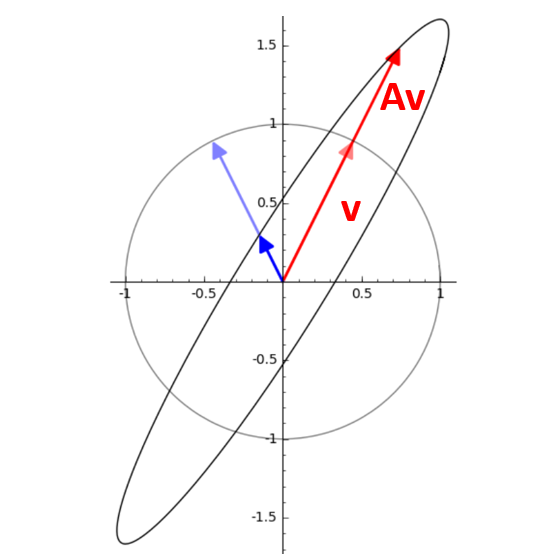
\includegraphics[keepaspectratio, scale=0.3]{pic/eigenvetor-eigenvalue-idea.png} \caption{\href{https://mathformachines.com/posts/eigenvalues-and-singular-values/}{Figure reference}}
            \end{center}
        \end{figure}
    \end{minipage}
\end{frame}

\begin{frame}{How to Find Eigenvalues and Eigenvectors?}
    \begin{itemize}
        \item We know that
        $$Av = \lambda v$$
        \item So
        $$Av - \lambda v  = 0$$
        $$(A - \lambda I)v = 0$$
        \item $v$ can not be zero, so:
        $$det(A - \lambda I) = 0$$
        \item Solve for $\lambda$
        \item Substitute $\lambda$ back into the equation $Av = \lambda v$ to find $v$.
    \end{itemize}
\end{frame}

\begin{frame}{Numerical Example}
    \begin{itemize}
        \item Assume $A = \begin{pmatrix}  
4 & -5  \\
2 & -3 \\
\end{pmatrix} $
    \item $A - \lambda I =  ?$
    \end{itemize}
\end{frame}

\begin{frame}{Numerical Example (Continued)}
    \begin{itemize}
        \item Assume $A = \begin{pmatrix}  
4 & -5  \\
2 & -3 \\
\end{pmatrix} $
    \item $A - \lambda I =  \begin{pmatrix}  
4 - \lambda & -5  \\
2 & -3 - \lambda \\
\end{pmatrix}$
    \item Determinant $(A - \lambda I) = (4 - \lambda) (-3 - \lambda) + 10 = \lambda^2 - \lambda - 2$ 
    \end{itemize}
\end{frame}

\begin{frame}{Numerical Example (Continued)}
    \begin{itemize}
        \item Assume $A = \begin{pmatrix}  
4 & -5  \\
2 & -3 \\
\end{pmatrix} $
    \item $A - \lambda I =  \begin{pmatrix}  
4 - \lambda & -5  \\
2 & -3 - \lambda \\
\end{pmatrix}$
    \item Determinant $(A - \lambda I) = (4 - \lambda) (-3 - \lambda) + 10 = \lambda^2 - \lambda - 2$ 
    \item $\lambda = -1$ or $\lambda = 2$
    \item $
\lambda_1 = -1 : \quad (A - \lambda_1 I) v_1 = 
\begin{bmatrix}
5 & -5 \\
2 & -2
\end{bmatrix}
\begin{bmatrix}
y \\
z
\end{bmatrix}
=
\begin{bmatrix}
0 \\
0
\end{bmatrix} \quad \rightarrow v_1 = \begin{bmatrix}
1 \\
1
\end{bmatrix}
$
    \item $
\lambda_2 = 2 : \quad (A - \lambda_2 I) v_2 = 
\begin{bmatrix}
2 & -5 \\
2 & -5
\end{bmatrix}
\begin{bmatrix}
y \\
z
\end{bmatrix}
=
\begin{bmatrix}
0 \\
0
\end{bmatrix} \quad \rightarrow v_2 = \begin{bmatrix}
5 \\
2
\end{bmatrix}
$
    \end{itemize}
\end{frame}

\begin{frame}{Visualization}
    \begin{itemize}
        \item $Av = \lambda v$
        \begin{figure}[htpb]
            \begin{center}
                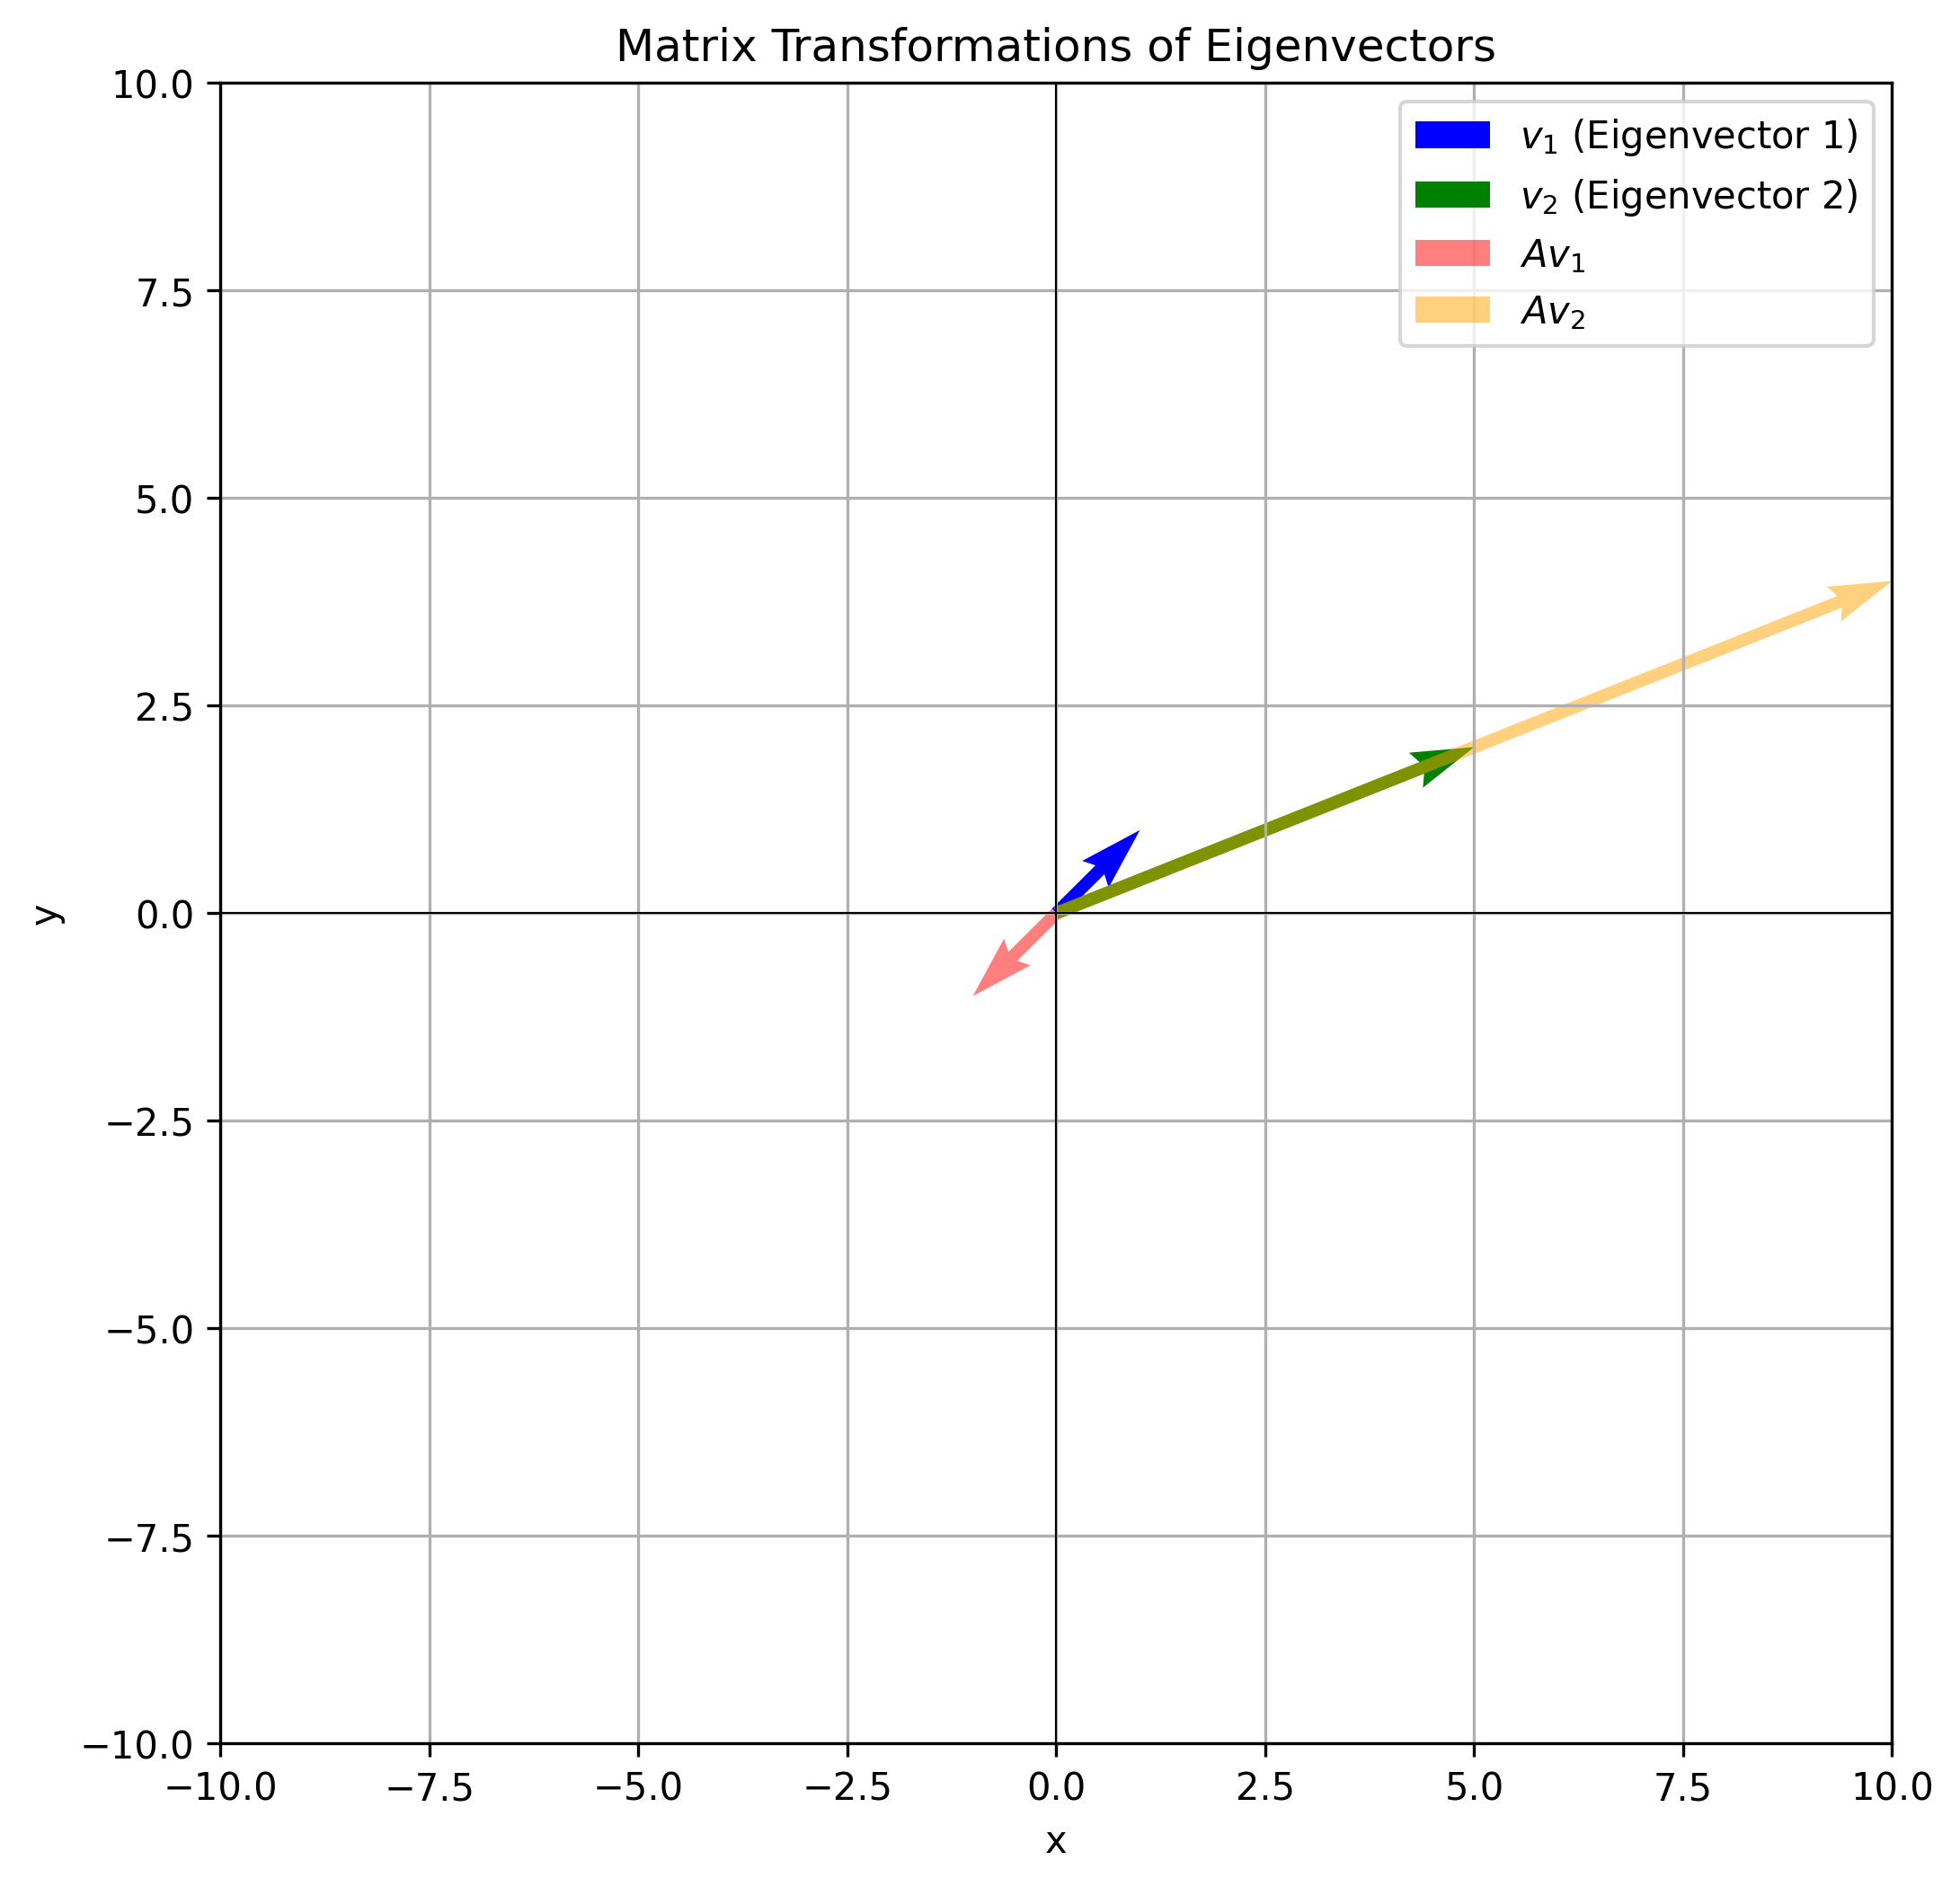
\includegraphics[keepaspectratio, scale=0.37]{pic/matrix_transformations.png}
            \end{center}
        \end{figure}
    \end{itemize}
\end{frame}

\subsubsection{Sample Covariance Matrix}

\begin{frame}{What is Covariance?}
    \begin{itemize}
        \item Covariance is a measure of how much two random features vary together.
        \item $ \text{Cov}(X, Y) = \mathbb{E}[(X - \mathbb{E}[X])(Y - \mathbb{E}[Y])] = \mathbb{E}[(Y - \mathbb{E}[Y]) (X - \mathbb{E}[X])] = \text{Cov}(Y, X)$
        \item So covariance is symmetric.
        \item Such as heights and weights of individuals.

    \end{itemize}
\end{frame}

% \begin{frame}{What is Covariance?}
%     \begin{itemize}         
%         \item Covariance shows the correlation between variables.
%         \begin{figure}[htpb]
%             \begin{center}
%                   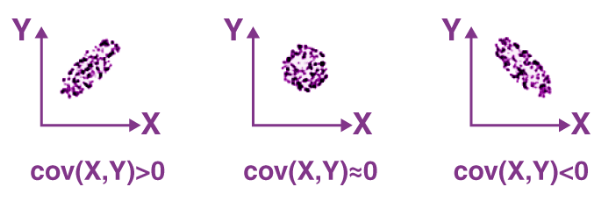
\includegraphics[keepaspectratio, scale=0.8]{pic/covariance.PNG} \caption{\href{https://byjus.com/maths/covariance/}{Figure reference}}
%             \end{center}
%         \end{figure}
%     \end{itemize}
% \end{frame}

\begin{frame}{What is a Covariance Matrix?}
    \begin{itemize}         
        \item A \textbf{covariance matrix} generalizes the concept of covariance to multiple features.
        
\item For a random vector $\mathbf{F} = [F_1, F_2, \dots, F_d]$:

$$
\Sigma = 
\begin{pmatrix}
\text{Var}(F_1) & \text{Cov}(F_1, F_2) & \cdots & \text{Cov}(F_1, F_d) \\
\text{Cov}(F_2, F_1) & \text{Var}(F_2) & \cdots & \text{Cov}(F_2, F_d) \\
\vdots & \vdots & \ddots & \vdots \\
\text{Cov}(F_d, F_1) & \text{Cov}(F_d, F_2) & \cdots & \text{Var}(F_d)
\end{pmatrix}
$$

\item The diagonal elements are the variances, and off-diagonal elements are covariances.
    \end{itemize}
\end{frame}


\begin{frame}{Covariance Matrix Example}
    \begin{itemize}         
        \item Suppose there is two feature covariance matrix:
$$
\Sigma = 
\begin{pmatrix}
a & b  \\
c & d 
\end{pmatrix} = \begin{pmatrix}
a & b   \\
b & d 
\end{pmatrix}
$$

        \item Why $b = c $?
        \item What is the relation between $a$, $b$, and $d $?
    \end{itemize}
\end{frame}

\begin{frame}{Covariance Matrix Example}
    \begin{itemize}         
        \item If $\Sigma = 
\begin{pmatrix}
a & 0  \\
0 & a 
\end{pmatrix}$, then:
        \begin{figure}[htpb]
            \begin{center}
         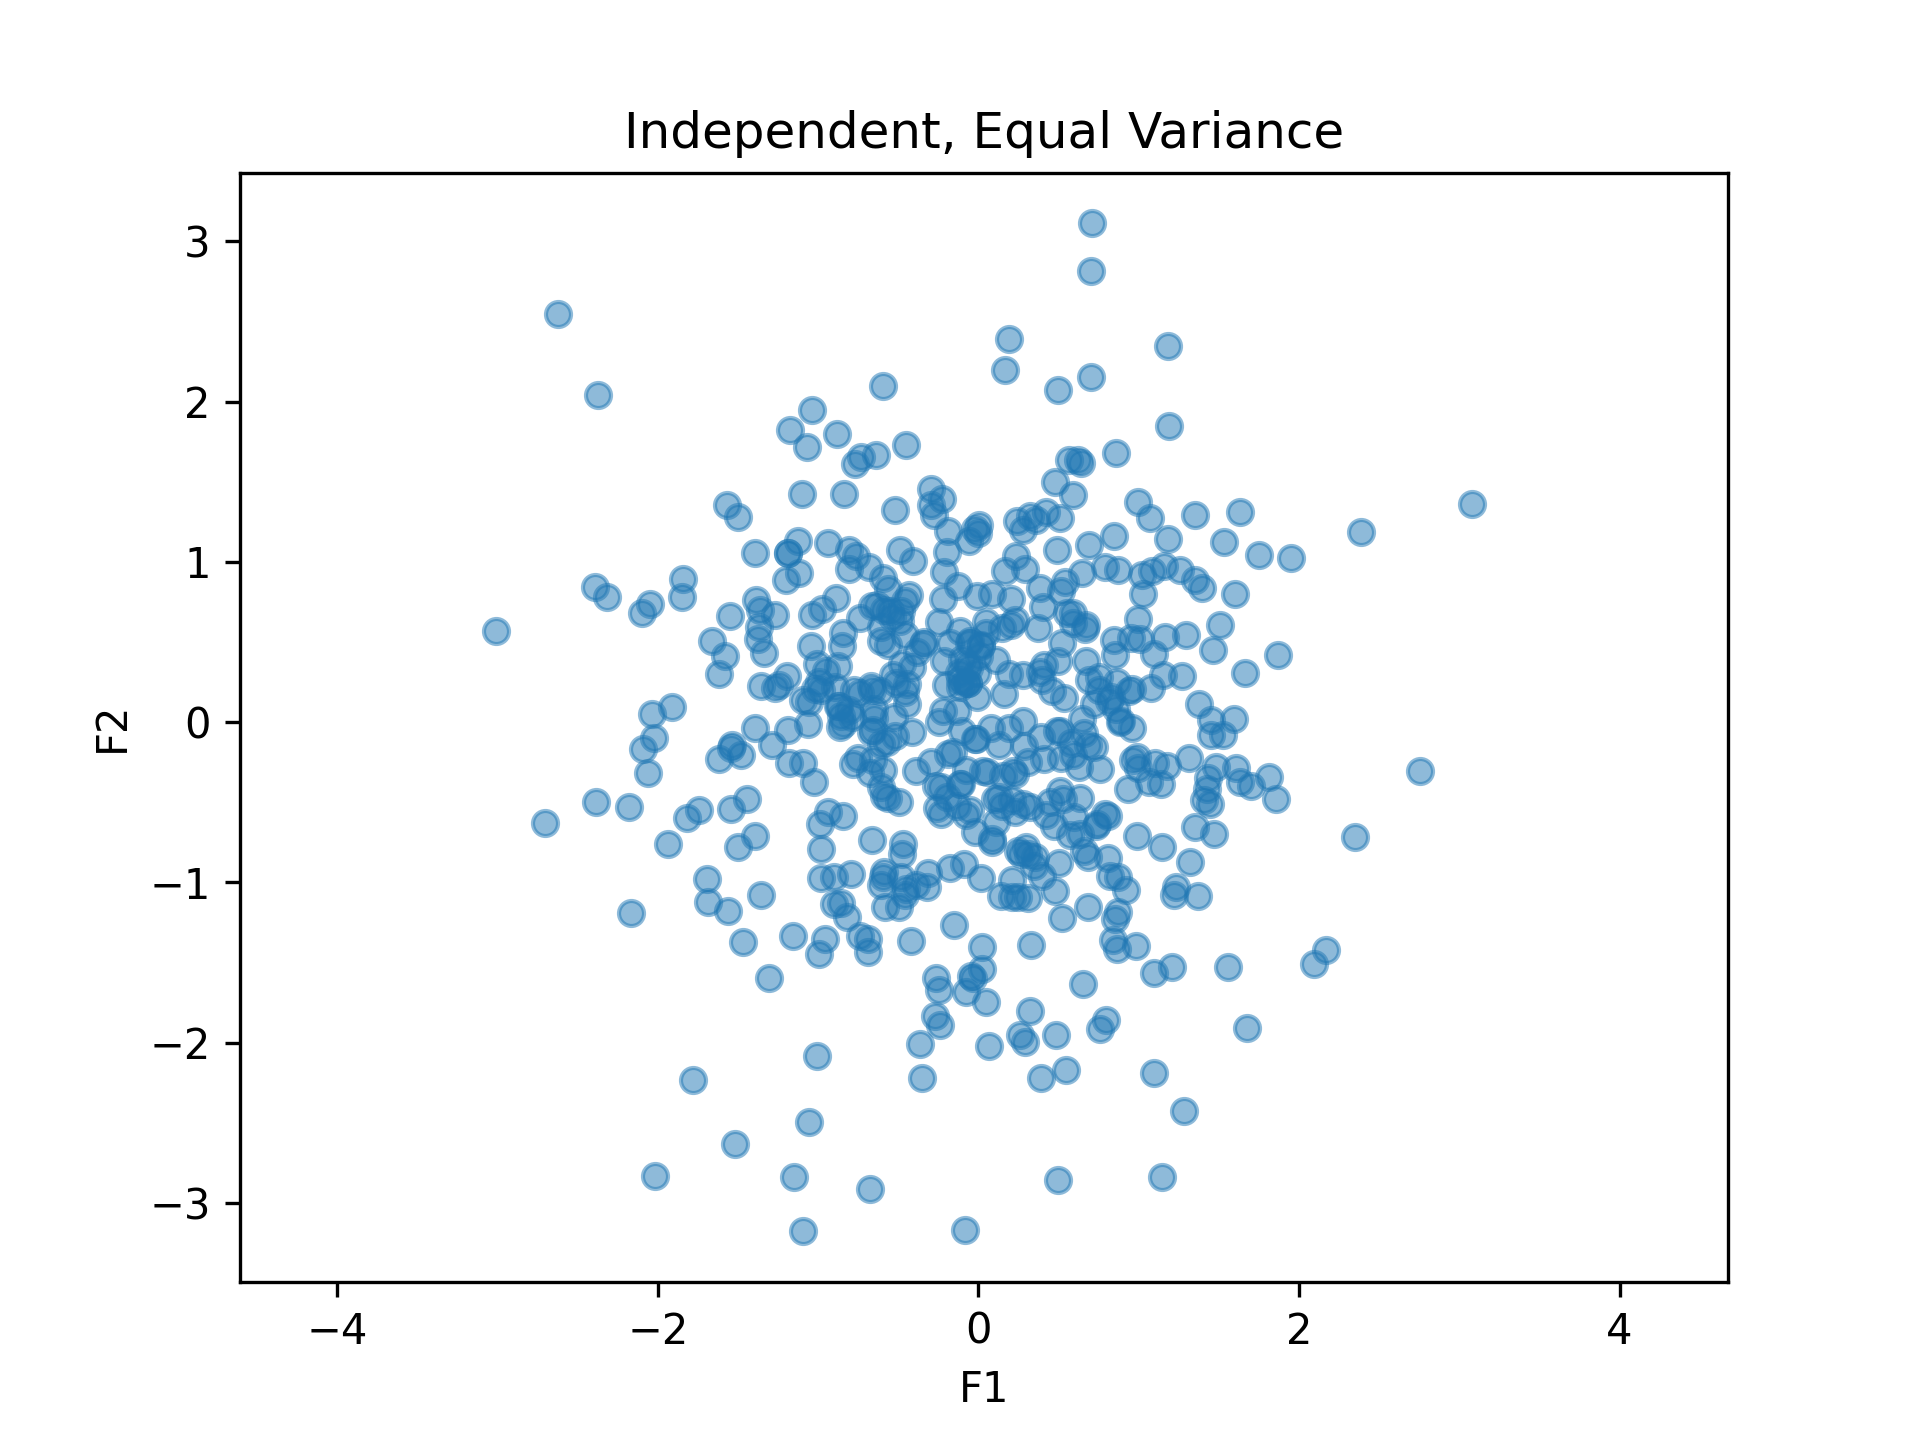
\includegraphics[keepaspectratio, scale=0.5]{pic/independent_equal_variance.png}
            \end{center}
        \end{figure}
    \end{itemize}
\end{frame}


\begin{frame}{Covariance Matrix Example}
    \begin{itemize}         
        \item If $\Sigma = 
\begin{pmatrix}
a & 0  \\
0 & d 
\end{pmatrix}$ and $a > d$, then:
        \begin{figure}[htpb]
            \begin{center}
         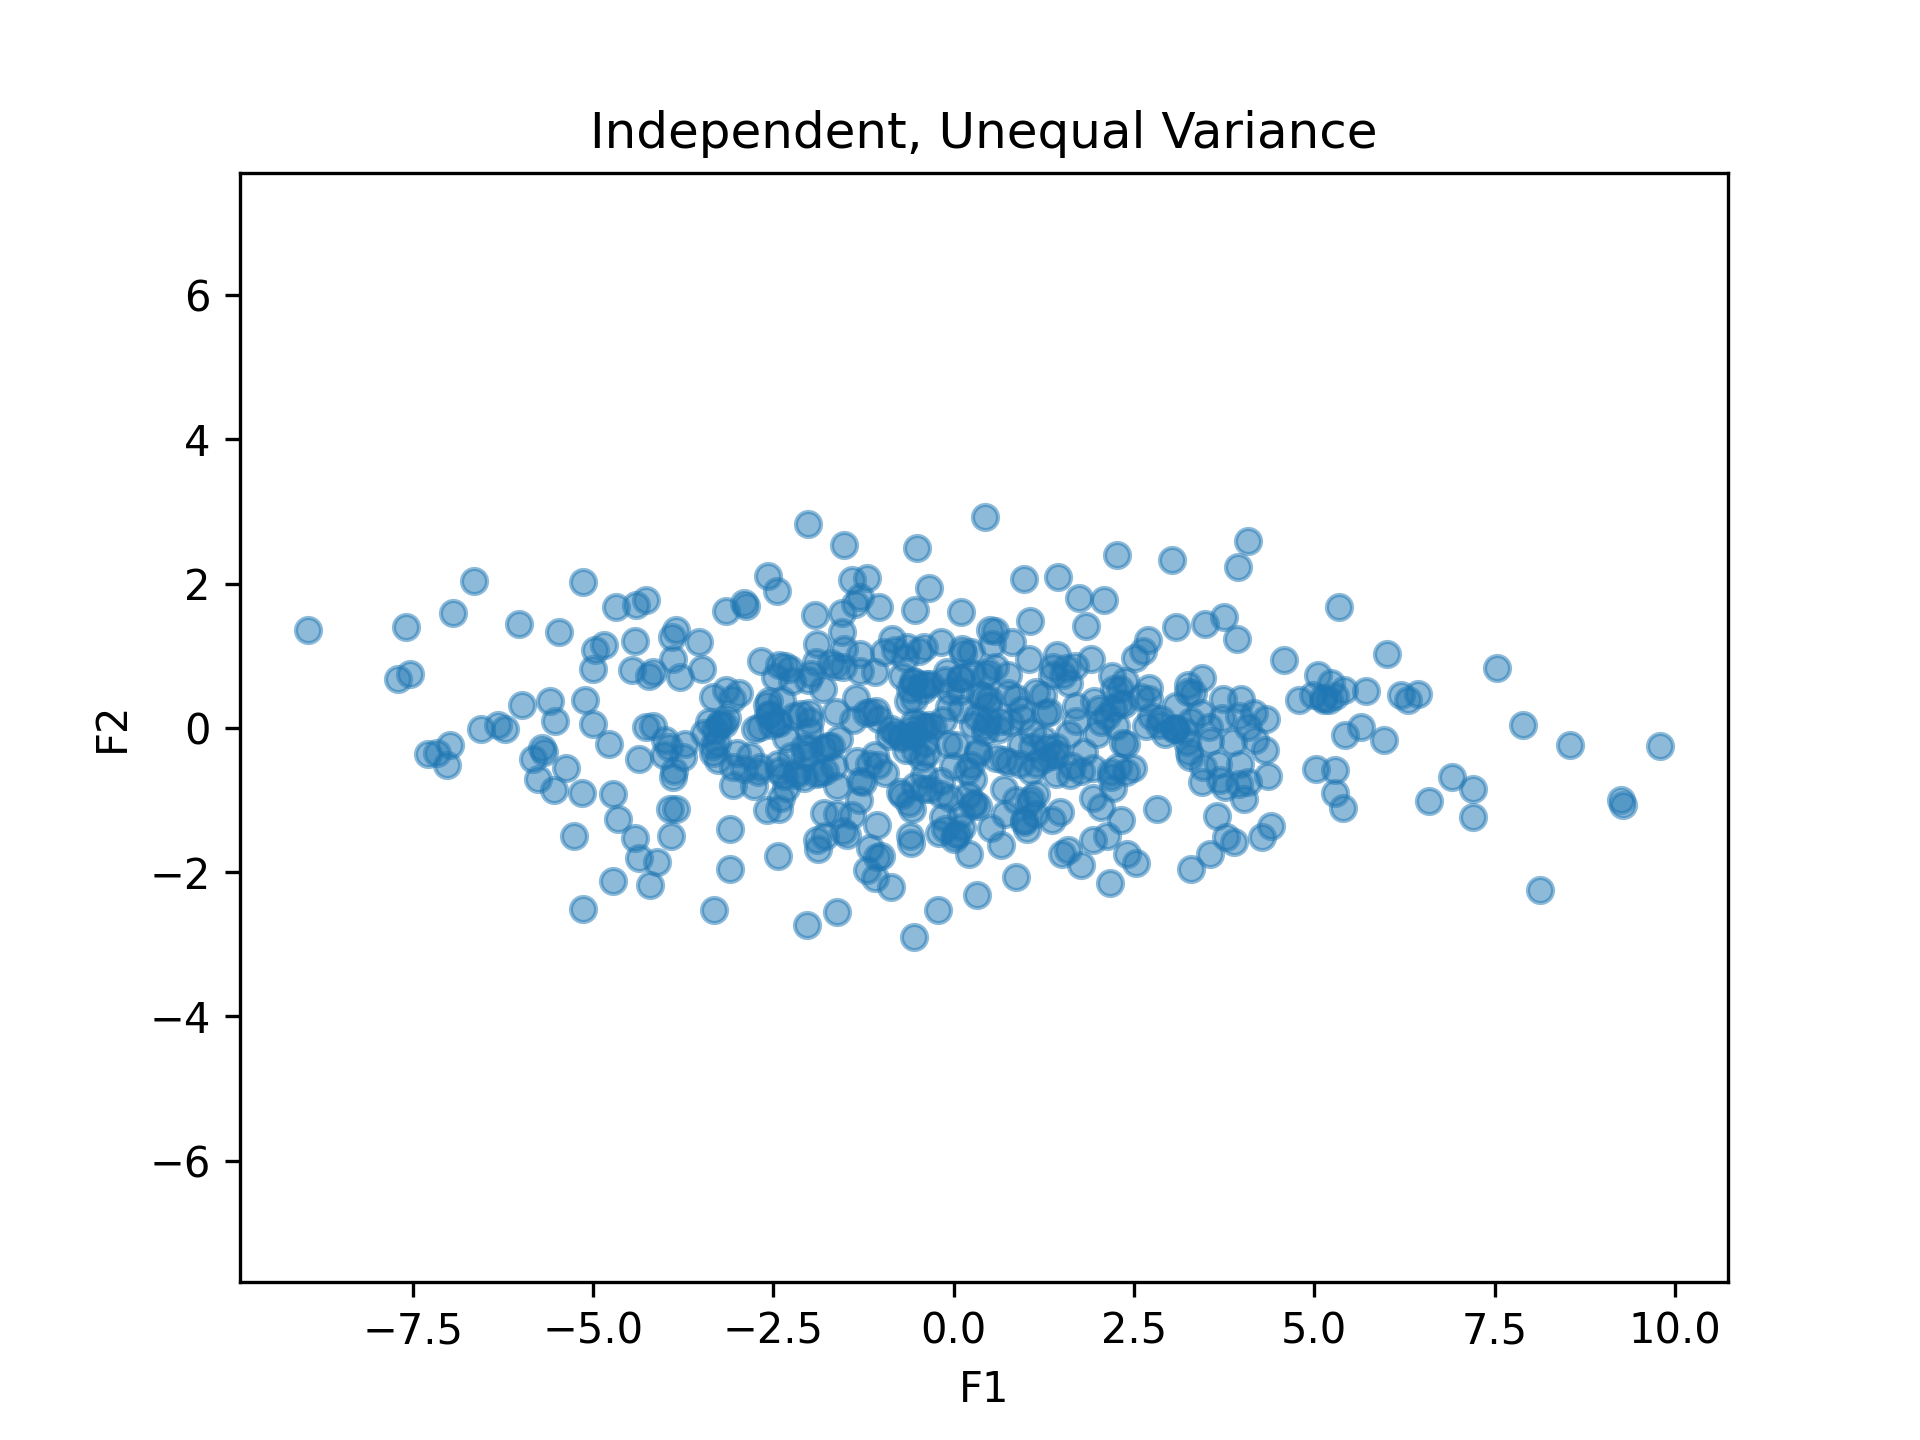
\includegraphics[keepaspectratio, scale=0.5]{pic/independent_unequal_variance.png}
            \end{center}
        \end{figure}
    \end{itemize}
\end{frame}

\begin{frame}{Covariance Matrix Example}
    \begin{itemize}         
        \item If $\Sigma = 
\begin{pmatrix}
a & b  \\
b & d 
\end{pmatrix}$, $a > d$, and $b > 0$, then: 
        \begin{figure}[htpb]
            \begin{center}
         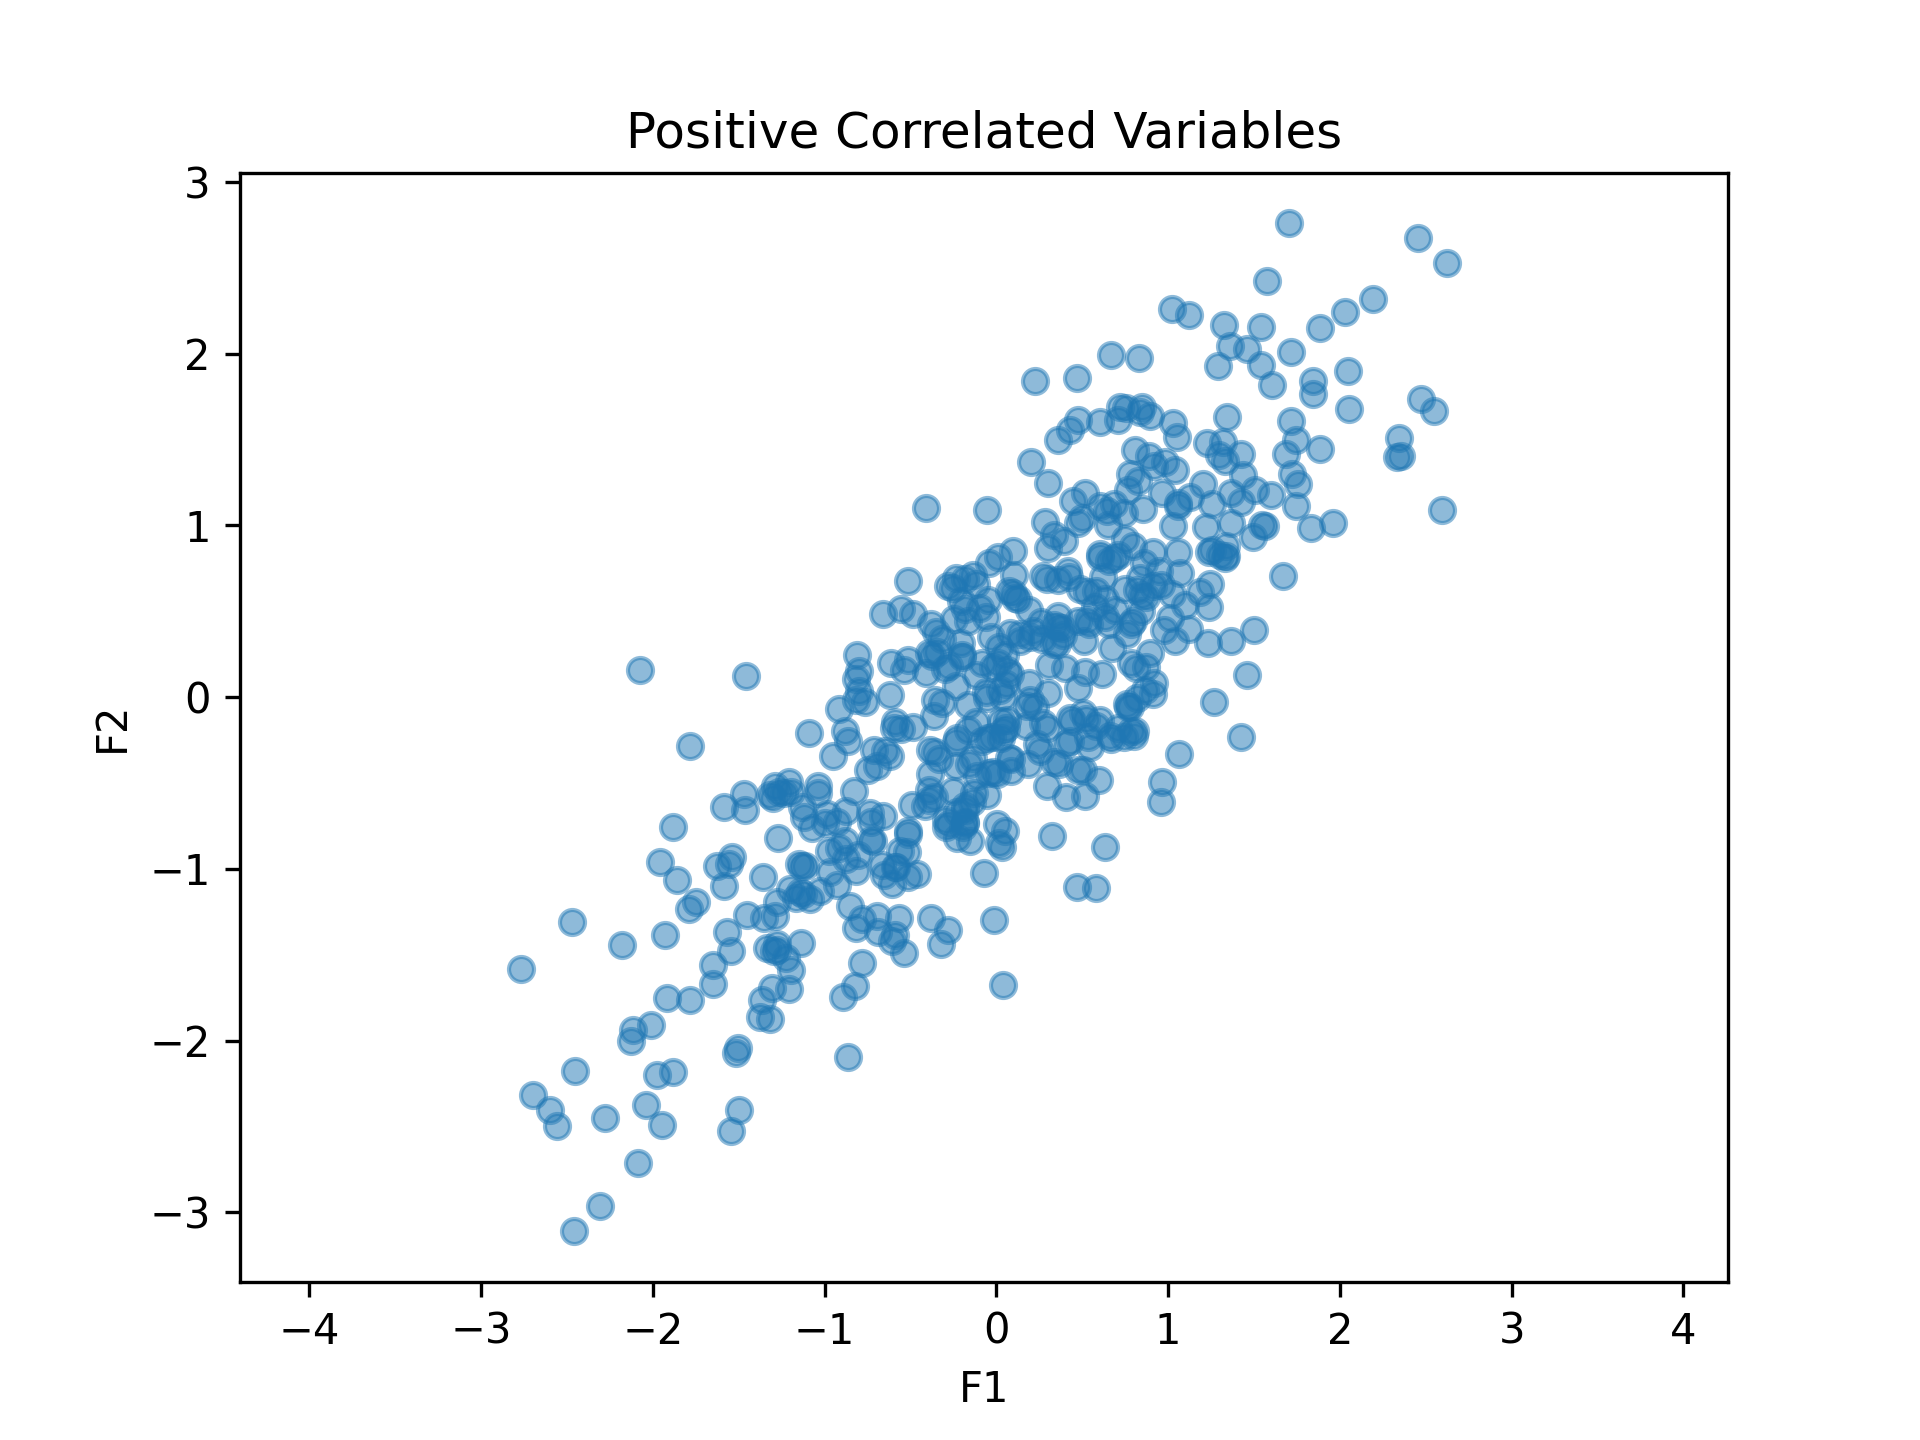
\includegraphics[keepaspectratio, scale=0.5]{pic/positive_correlated_variables.png}
            \end{center}
        \end{figure}
    \end{itemize}
\end{frame}


\begin{frame}{Covariance Matrix Example}
    \begin{itemize}         
        \item If $\Sigma = 
\begin{pmatrix}
a & b  \\
b & d 
\end{pmatrix}$, $a > d$, and $b < 0$, then: 
        \begin{figure}[htpb]
            \begin{center}
         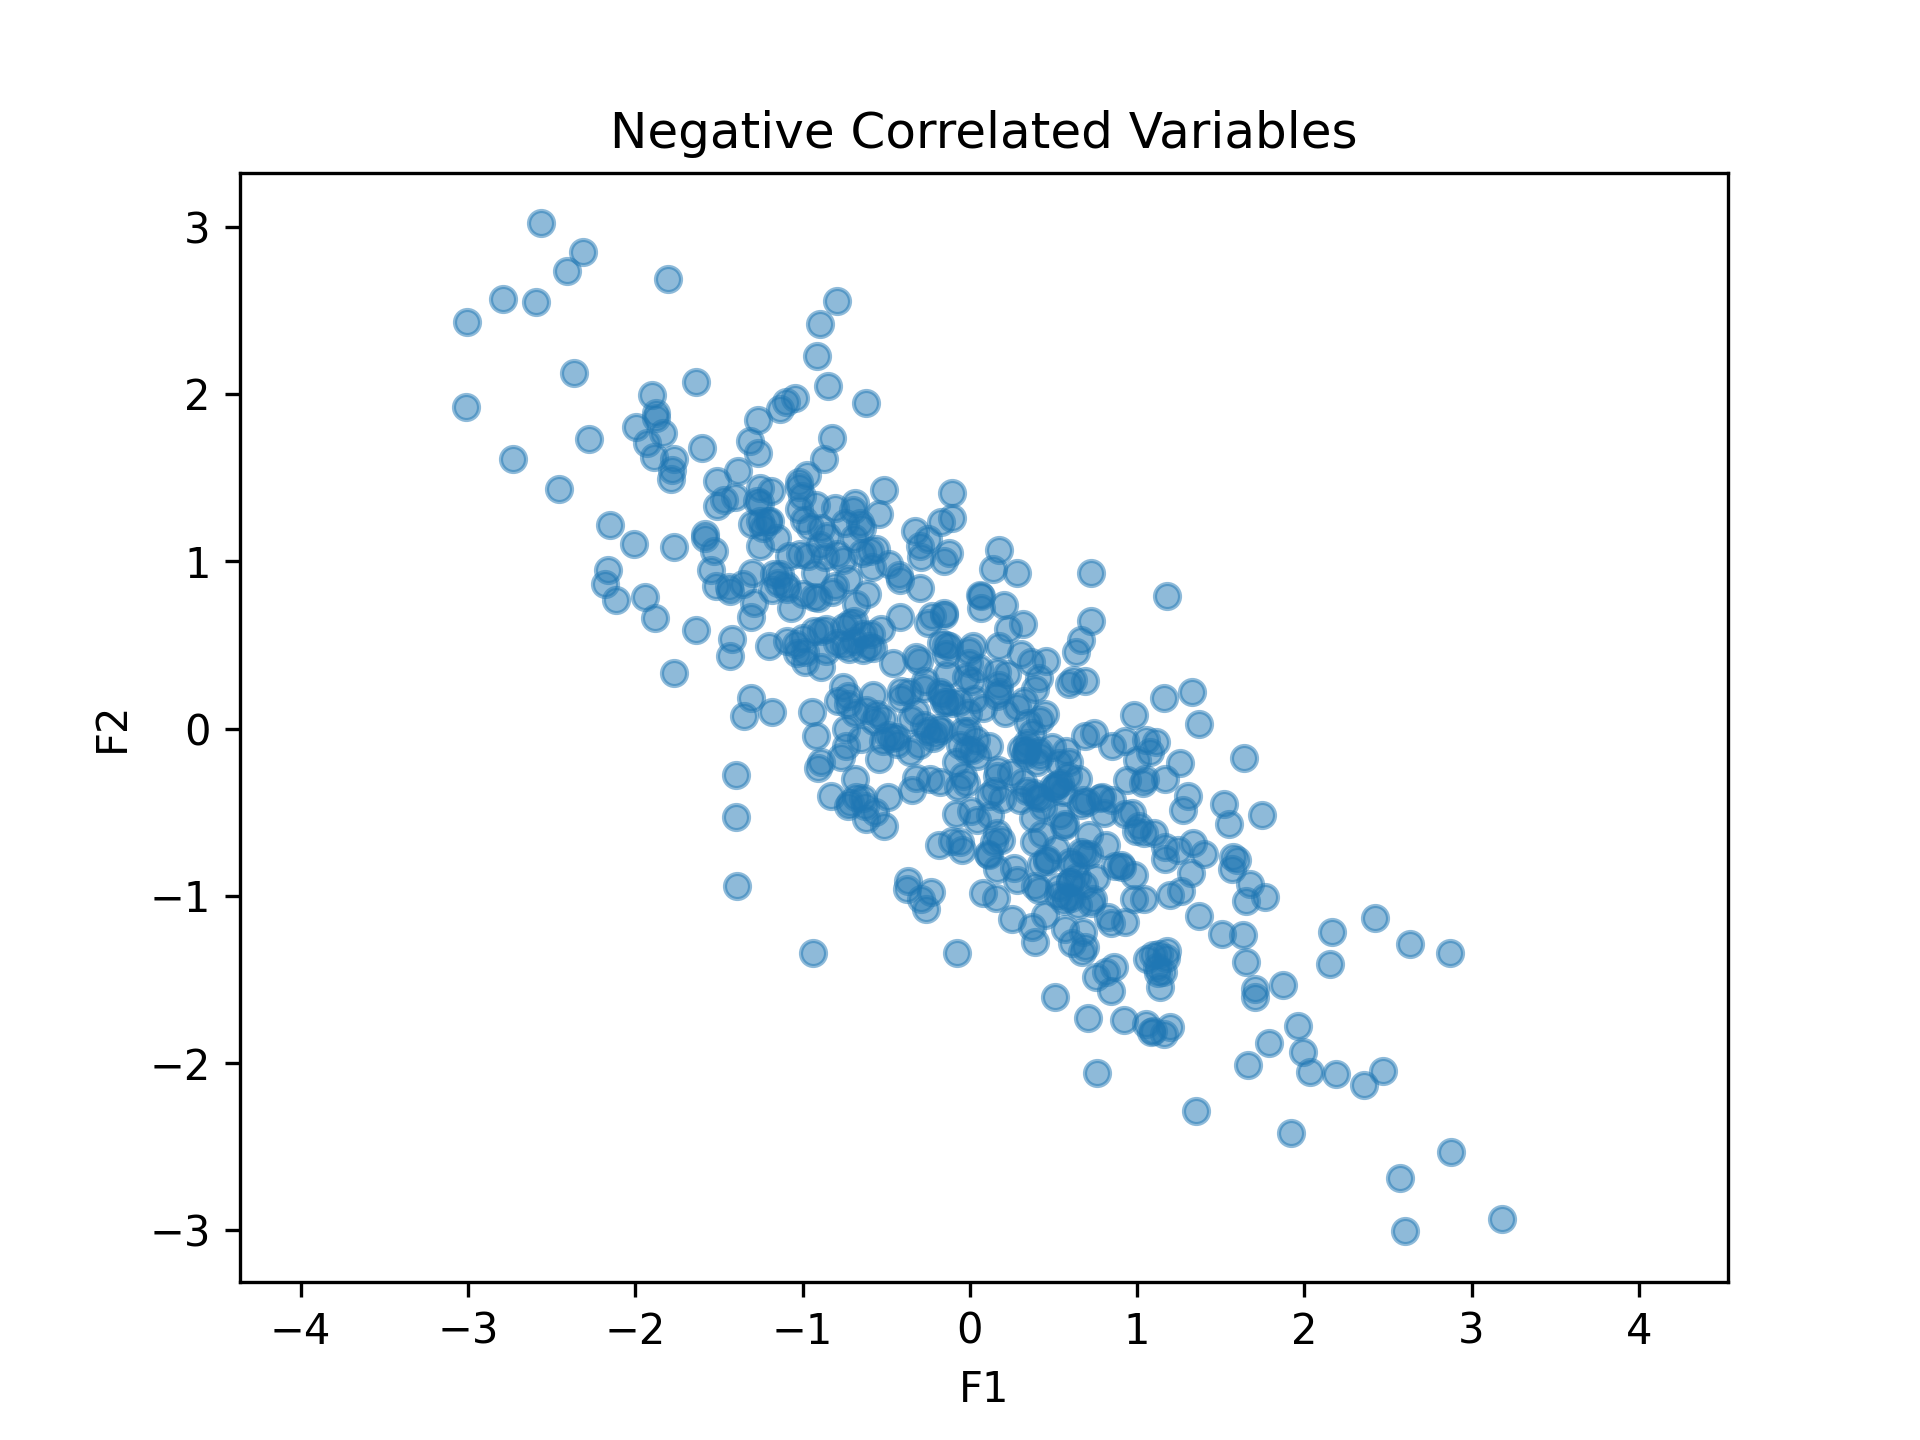
\includegraphics[keepaspectratio, scale=0.5]{pic/negative_correlated_variables.png}
            \end{center}
        \end{figure}
    \end{itemize}
\end{frame}


\begin{frame}{Sample Covariance Matrix}
    \begin{itemize}         
        \item In practice, we estimate covariance from sample data.
        \item \textbf{Sample Covariance Matrix}: Given $N$ samples of $d$ features, the sample covariance matrix $\Sigma$ is:
        $$
        \Sigma_{d\times d} = \frac{1}{N-1} \sum_{i=1}^{N} (X_i - \bar{X})(X_i - \bar{X})^T
        $$
        \item Where $X_i$  is the i-th sample, and $\bar{X}_{d \times 1}$
  is the mean of the samples.
    \end{itemize}
\end{frame}


% \begin{frame}{Deriving the Sample Covariance Matrix}
%     \begin{itemize}         
%         \item  Center the data by subtracting the mean of each variable from the corresponding observations:
%         $$X_centered = X - \bar{X} $$
%         \item Multiply the centered data by its transpose to compute the covariance.
%     \end{itemize}
% \end{frame}



\begin{frame}{Example Calculation of Sample Covariance Matrix}
    \begin{itemize}         
        \item Suppose we have the following three samples each one having two features F$_1$ and F$_2$:
\begin{center}
     \begin{tabular}{|c|c|c|}
        \hline
        \textbf{Sample} & \textbf{F$_1$} & \textbf{F$_2$} \\
        \hline
        $X_1$ & 3 & 3 \\
        \hline
        $X_2$ & 4 & 7 \\
        \hline
        $X_3$ & 5 & 8 \\
        \hline
        $\bar{X}$ & 4 & 6 \\
        \hline
        \end{tabular}
\end{center}
     
     $$\Sigma =  \frac{1}{N-1} \sum_{i=1}^{N} (X_i - \bar{X})(X_i - \bar{X})^T =  \frac{1}{2} (\begin{pmatrix}
1 & 3  \\
3 & 9 
\end{pmatrix}  + \begin{pmatrix}
0 & 0  \\
0 & 1 
\end{pmatrix} + \begin{pmatrix}
1 & 2  \\
2 & 4 
\end{pmatrix}) =  \begin{pmatrix}
1 & 2.5  \\
2.5 & 7 
\end{pmatrix} $$
    \end{itemize}
\end{frame}

% \begin{frame}{Properties of the Covariance Matrix}
%     \begin{itemize}         
%       \item \textbf{Symmetry:} $\Sigma$ is always symmetric: $\Sigma = \Sigma^T$
%       \item \textbf{Positive Semi-Definite:} For any vector $v$, $v\Sigma v^T \geq 0$
%       \item \textbf{Diagonal Elements:}         Variances of each variable.
%       \item \textbf{Off-diagonal Elements:} Covariances between variables.
%     \end{itemize}
% \end{frame}

\subsubsection{Lagrangian multiplier}

% \begin{frame}{Optimization with Constraints}
%     \begin{itemize}
%         \item Optimization seeks to find maximum or minimum values of a function.
%         \item In constrained optimization, the function is subject to one or more restrictions.
%     \end{itemize}
% \end{frame}


% \begin{frame}{Lagrange Multiplier: The Concept}
%     \begin{itemize}
%         \item The Lagrange multiplier is a method used to find local maxima or minima of a function $f(x)$ subject to equality constraints $g(x) = 0$.
%         \item It helps in solving optimization problems by converting them into a system of equations.
        
%     \end{itemize}
% \end{frame}

\begin{frame}{Lagrange Multiplier: Geometrical Interpretation}
    \begin{itemize}
        \item We want to maximize $f(x)$ subject to $g(x) = 0$.
        \item The optimal point occurs where the gradient of $f(x)$ is proportional to the gradient of $g(x)$ (i.e., they are aligned or in opposite directions). 
     \begin{figure}[htpb]
            \begin{center}
         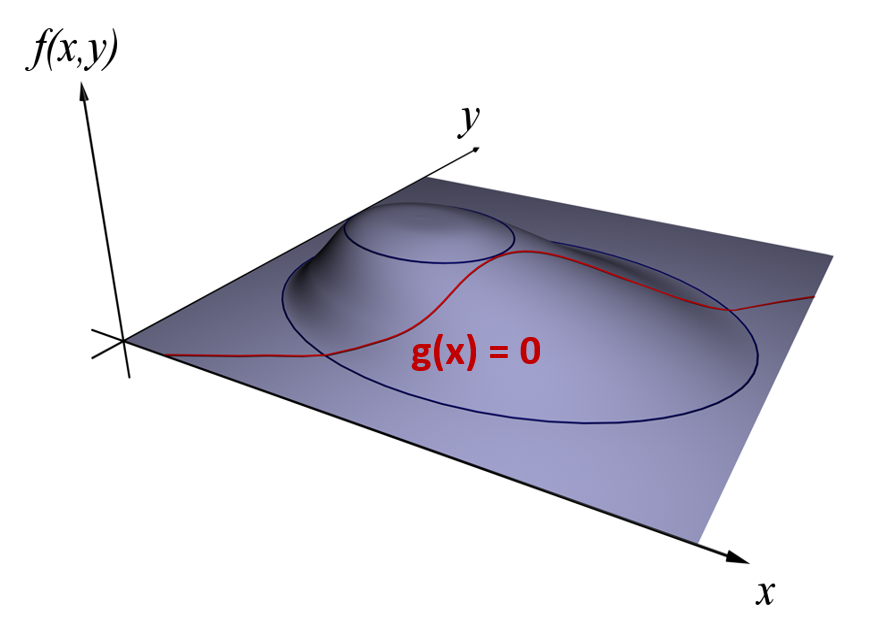
\includegraphics[keepaspectratio, scale=0.4]{pic/lagrange3d.png}
         \caption{\href{https://www.khanacademy.org/math/multivariable-calculus/applications-of-multivariable-derivatives/constrained-optimization/a/lagrange-multipliers-examples}{Figure reference}}
            \end{center}
        \end{figure}
    \end{itemize}
\end{frame}

\begin{frame}{Lagrange Multiplier Method}
    \begin{itemize}
        \item Combine the objective function and the constraint using the Lagrange function:
        $$\mathcal{L}(x, \lambda) = f(x) + \lambda g(x)$$
        \item Solve the system of equations:
        $$\nabla \mathcal{L}(x, \lambda) = 0$$
        \item Where:
        \begin{itemize}
            \item $\mathcal{L}$ is  lagrangian
            \item $\lambda$ is lagrange multiplier
            \item $g(x)$ is equality constraint
            \item $f(x)$ is function
        \end{itemize}
    \end{itemize}
\end{frame}


% \begin{frame}{The Lagrangian Function}
%     \begin{itemize}
%         \item The Lagrangian is a function that incorporates both the objective function and the constraint.
%         \item It allows us to find critical points where both the function and the constraint behave optimally.
%         $$ \mathcal{L}(x_1, x_2, \cdots, \lambda) = f(x_1, x_2, \cdots, x_n) - \lambda g(x_1, x_2, \cdots, x_n)$$
%     \end{itemize}
% \end{frame}


% \begin{frame}{The Lagrangian Function}
%     \begin{enumerate}
%         \item Write the Lagrangian function $\mathcal{L}(x, \lambda) = f(x) - \lambda g(x)$
%          \item Take partial derivatives \( \frac{\partial \mathcal{L}}{\partial x_i} \) and \( \frac{\partial \mathcal{L}}{\partial \lambda} \).
%          \item Solve the system of equations \( \nabla \mathcal{L} = 0 \).
%          \item Find \( x \) and \( \lambda \), then evaluate \( f(x) \) for optimal values.
%     \end{enumerate}
% \end{frame}

\begin{frame}{Example Problem}
\begin{itemize}
    \item \text{Maximize:}
        \[
 \quad f(x_1, x_2) = x_1 + x_2
\]
    \item Subject to:
    \[
x_1^2 + x_2^2 = 1
\]
    \item Lagrangian:
    \[
L(x_1, x_2, \lambda) = x_1 + x_2 - \lambda (x_1^2 + x_2^2 - 1)
\]
    \item Partial derivatives:
    \[
\begin{cases}
\frac{\partial L}{\partial x_1} = 1 - 2\lambda x_1 = 0 \\
\frac{\partial L}{\partial x_2} = 1 - 2\lambda x_2 = 0 \\
\frac{\partial L}{\partial \lambda} = -(x_1^2 + x_2^2 - 1) = 0
\end{cases}
\]
\end{itemize}
\end{frame}

\begin{frame}{Example Problem (Continued)}
\begin{itemize}
    \item Solving:
\[
\begin{cases}
\lambda x_1 = \dfrac{1}{2} \\
\lambda x_2 = \dfrac{1}{2} \\
x_1^2 + x_2^2 = 1
\end{cases}
\]
    \item Since \(\lambda x_1 = \lambda x_2\), then \(x_1 = x_2\).
    \item Substitute \(x_1 = x_2\) into the constraint:
    \[
2x_1^2 = 1 \implies x_1 = \pm \dfrac{1}{\sqrt{2}}
\]
    \item Optimal solution:
\[
x_1 = x_2 = \dfrac{1}{\sqrt{2}}, \quad f_{\text{max}} = x_1 + x_2 = \sqrt{2}
\]
\end{itemize}

\end{frame}

% \begin{frame}{Example Problem}
%     \begin{enumerate}
%         \item Maximize following function with given constraints:
%         $$f(x_1, x_2) = x_1 + x_2$$
%         $$g(x, y) = x_1^2 + x_2^2 - 1 = 0$$
%         \item Solution of the following problem:
%         $$\mathcal{L}(x, y, \lambda) = xy - \lambda(x^2 + y^2 - 1)$$
%         \item Take derivative of $x$, $y$, and $\lambda$:
%         $$\frac{\partial \mathcal{L}}{\partial x} = y - 2 \lambda x = 0$$
%         $$\frac{\partial \mathcal{L}}{\partial y} = x - 2 \lambda y = 0$$
%         $$\frac{\partial \mathcal{L}}{\partial \lambda} = -(x^2 + y^2 - 1) = 0$$

%     \end{enumerate}
% \end{frame}

% \begin{frame}{Example Problem (Continued)}
%     \begin{itemize}
%         \item After solving above system of equations, we have:
%         $$\lambda = \pm \frac{1}{2}$$
%         \item Case 1: $\lambda = \frac{1}{2}$:
%         $$y = 2 \times \frac{1}{2} x \rightarrow y = x$$
%         $$x^2 + x^2 = 1 \rightarrow x = \pm \frac{1}{\sqrt{2}}$$
%         $$(x, y) = \left( \frac{1}{\sqrt{2}}, \frac{1}{\sqrt{2}} \right) \text{ or } \left( \frac{-1}{\sqrt{2}}, \frac{-1}{\sqrt{2}} \right)$$
%     \end{itemize}
% \end{frame}


% \begin{frame}{Example Problem (Continued)}
%     \begin{itemize}
%         \item Case 2: $\lambda = -\frac{1}{2}$:
%         $$y = 2 \times -\frac{1}{2} x \rightarrow y = -x$$
%         $$x^2 + x^2 = 1 \rightarrow x = \pm \frac{1}{\sqrt{2}}$$
%         $$(x, y) = \left( \frac{1}{\sqrt{2}}, \frac{-1}{\sqrt{2}} \right) \text{ or } \left( \frac{-1}{\sqrt{2}}, \frac{1}{\sqrt{2}} \right)$$
        
%     \end{itemize}
% \end{frame}

% \begin{frame}{Example Problem (Continued)}
%     \begin{itemize}
%         \item Now, we should evaluate the results:
%         \begin{itemize}
%             \item If $(x, y) = \left( \frac{1}{\sqrt{2}}, \frac{1}{\sqrt{2}} \right)$, then $f(x, y) = \frac{1}{2}$
%             \item If $(x, y) = \left( \frac{-1}{\sqrt{2}}, \frac{-1}{\sqrt{2}} \right)$, then $f(x, y) = \frac{1}{2}$
%             \item If $(x, y) = \left( \frac{-1}{\sqrt{2}}, \frac{1}{\sqrt{2}} \right)$, then $f(x, y) = \frac{-1}{2}$
%             \item If $(x, y) = \left( \frac{1}{\sqrt{2}}, \frac{-1}{\sqrt{2}} \right)$, then $f(x, y) = \frac{-1}{2}$
%         \end{itemize}
%         \item So, when $(x, y) = \left( \frac{1}{\sqrt{2}}, \frac{1}{\sqrt{2}} \right)$ or $\left( \frac{-1}{\sqrt{2}}, \frac{-1}{\sqrt{2}} \right)$, $f(x, y)$ maximizes according to constraints.
%     \end{itemize}
% \end{frame}


% \begin{frame}{Geometrical Interpretation}
%     \begin{itemize}
%         \item   The gradient of the objective function $\nabla f(x, y)$ is parallel to the gradient of the constraint $\nabla g(x, y)$.
%         \item This means the constraint \textbf{touches} the level curve of the objective function at optimal points.
%         \begin{figure}[htpb]
%             \begin{center}
%          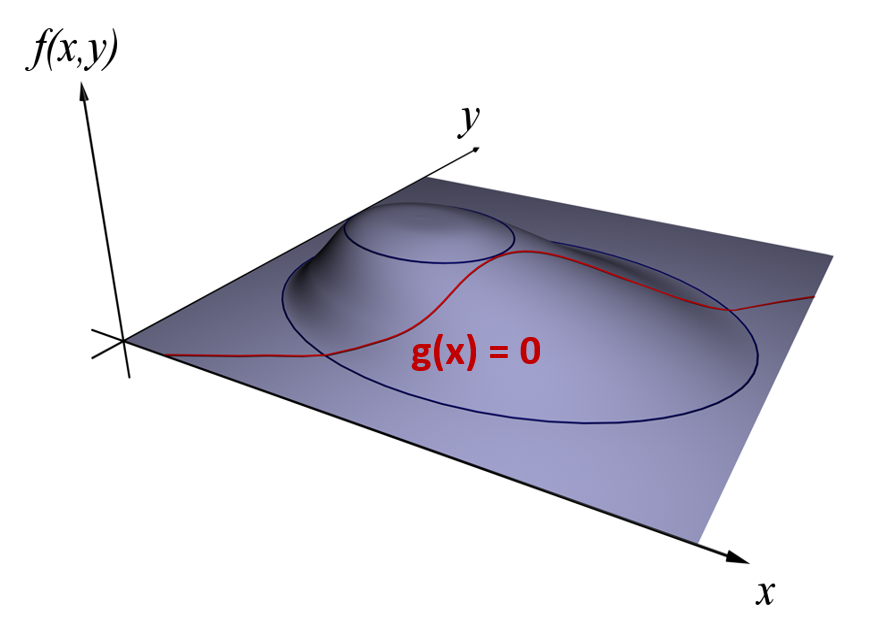
\includegraphics[keepaspectratio, scale=0.2]{pic/lagrange3d.png}
%          \caption{\href{https://www.khanacademy.org/math/multivariable-calculus/applications-of-multivariable-derivatives/constrained-optimization/a/lagrange-multipliers-examples}{Figure reference}}
%             \end{center}
%         \end{figure}
%     \end{itemize}
% \end{frame}


\begin{frame}{Generalization to Multiple Constraints}
    \begin{itemize}
    \item The Lagrange multiplier method can be extended to cases with more than one constraint.
    \item For constraints $g_1(x) = 0, g_2(x) = 0, \dots, g_m(x) = 0$, the Lagrangian becomes:
    \[
    \mathcal{L}(x, \lambda_1, \lambda_2, \dots) = f(x) - \lambda_1 g_1(x) - \lambda_2 g_2(x) - \dots
    \]
    \end{itemize}
\end{frame}


% \begin{frame}{Algorithms}
%     \begin{itemize}
%         \item Algorithm 1: sequential
%         \item Algorithm 2: sample covariance matrix
%     \end{itemize}
% \end{frame}

% \subsection{Sequential Algorithm}

% \begin{frame}{Sequential Algorithm}

%         \begin{itemize}
%             \item Find directions with the maximum variations
%              $$
%         \argmax_{v_1} \frac{1}{N} \sum_{n=1}^{N} (v_1^T x_n)^2 = \frac{1}{N} \sum_{n=1}^{N} v_1^T (x_n x_n^T) v_1 = v_1^T \left( \frac{1}{N} \sum_{n=1}^{N}(x_n x_n^T) \right) v_1 = v_1^T S {v_1}
%         $$
%         $$ \text{s.t. } v_1^{T}{v_1}  = 1$$
%         \item $S$ is sample covariance matrix.
%         \item Using Lagrangian multiplier technique:
%         $$\nabla \mathcal{L}(x_1, \lambda_1) = v_1^T S v_1 + \lambda (1 - v_1^Tv_1)$$
%         $$\frac{\partial \mathcal{L}}{\partial v_1} = 0 \rightarrow 2Sv_1 - 2\lambda_1 v_1 = 0$$
%         $$\rightarrow Sv_1 = \lambda_1 v_1$$
%         \end{itemize}
% \end{frame}

% \begin{frame}{Sequential Algorithm}
%     \begin{itemize}
%         \item Find directions with the maximum variations
%         $$
%         \argmax_{v_1} \frac{1}{N} \sum_{n=1}^{N} (v_1^T x_n)^2 = \frac{1}{N} \sum_{n=1}^{N} v_1^T (x_n x_n^T) v_1 = v_1^T \left( \frac{1}{N} \sum_{n=1}^{N}(x_n x_n^T) \right) v_1 = v_1^T S {v_1}
%         $$
%         $$ \text{s.t. } v_1^{T}{v_1}  = 1$$
%         \item   Using Lagrangian multiplier technique
%         $$ L(v_1, \lambda) = v_1^T S v_1 + \lambda (1 - v_1^T v_1) $$
%         $$ \frac{\partial L}{\partial v_1} = 0 \Rightarrow 2Sv_1 - 2\lambda v_1 = 0$$
%         $$ \Rightarrow Sv_1 = \lambda v_1 $$
%     \end{itemize}
% \end{frame}

% \begin{frame}{Sequential Algorithm}
%     \begin{itemize}
%         \item To find $v_2$, we maximize the variance of the projection in the residual subspace
% $$
% v_2 = \argmax_{v_2} \left( \frac{1}{N} \sum_{i=1}^{N} v_2^T\left( x_i - v_1^T x_i \right)^2 \right)
% $$
% $$ \text{s.t. } v_2^{T}{v_2}  = 1$$
%           \item To find $v_k$, we maximize the variance of the projection in the residual subspace
% $$
% v_k = \argmax_{v_k} \left( \frac{1}{N} \sum_{i=1}^{N} v_k^T\left( x_i - \sum_{j=1}^{k-1} v_j^T x_i \right)^2 \right)
% $$      
% $$\text{s.t. } v_k^{T}{v_k}  = 1$$
%     \end{itemize}
% \end{frame}

% \begin{frame}{Sequential Algorithm}
%     \begin{itemize}
%         \item Second view
%         \begin{itemize}
%             \item Find directions with the minimum reconstruction error 
%         \end{itemize}
%         $$
%         \min_{v1} \sum_{n=1}^{N} \lVert x_n - (v_{1}^{T} x_n)v_{1} \rVert_2^{2}
%         $$
%         $$ \text{s.t. } v_1^{T}{v_1}  = 1$$
%         \item Show this has an equal solution with the first view

%         \begin{figure}[htpb]
%             \begin{center}
%                 \includegraphics[keepaspectratio, scale=0.55]{pic/var_vs_rec.JPG}
%             \end{center}
%         \end{figure}

%     \end{itemize}
% \end{frame}


% \begin{frame}{Sequential Algorithm}
%     \begin{itemize}
%       \item As we have $S v_j = \lambda_j v_j$,

%     $$\Rightarrow \text{var}(v_j^T x) = v_j^T x x^{T} v_j =
%       v_j^T S v_j =
%       \lambda_j v_j^T v_j =
%       \lambda_j$$.
    
%     \item The variance along an eigenvector  $v_j \text{ equals the eigenvalue } \lambda_j. $
        
%     \end{itemize}
% \end{frame}

% \begin{frame}{Sequential Algorithm}
%     \begin{itemize}
%       \item Eigenvalues: $\lambda_1 \geq \lambda_2 \geq \lambda_3 \geq ... \geq 0 $
%         \begin{itemize}
%             \item The first PC, $v_1$, is the the eigenvector of the sample covariance matrix $S$ associated with the largest eigenvalue
%             \item The 2nd PC, $v_2$, is the the eigenvector of the sample covariance matrix $S$ associated with the second largest eigenvalue
%             \item And so on ...
%         \end{itemize}
%          \item To reduce the dimension of the data to $k$, we select eigenvectors with the top $k$ eigenvalues
        
%     \end{itemize}
% \end{frame}


\subsection{Sample Covariance Matrix Algorithm}

% \begin{frame}{Sample Covariance Matrix Algorithm}
%     \begin{itemize}
%         \item Given data ${x_1, …, x_n}$, compute covariance matrix $\Sigma$
%         $$\Sigma = \frac{1}{n - 1} \sum_{i=1}^{n} (x_i - \bar{x})(x_i - \bar{x})^T \text{ where }  \bar{x} = \frac{1}{n} \sum_{i=1}^{N} x_i $$
%         \item PCA basis vectors = the eigenvectors of $\Sigma$
%         \item Larger eigenvalue $\rightarrow$ more important eigenvectors
%     \end{itemize}
% \end{frame}

% \begin{frame}{Principal Component Analysis Review}
%     \begin{itemize}
%         \item Goal: Maximize the variance of the projected data.
%         \item Given a dataset \( X \in \mathbb{R}^{n \times d} \), where \( n \) is the number of samples and \( d \) is the number of features.
%         \item The data is centered, meaning the mean of each feature is 0.
%     \end{itemize}
% \end{frame}

% Slide 2 - Covariance Matrix Definition
% \begin{frame}{Covariance Matrix}
%     \begin{itemize}
%         \item The covariance matrix of the dataset \( X \) is defined as:
%         \[
%         \Sigma = \frac{1}{n} X^\top X \in \mathbb{R}^{d \times d}
%         \]
%         \item We seek a direction \( v \in \mathbb{R}^d \) such that \( \|v\| = 1 \), maximizing the variance of the projected data \( Xv \).
%     \end{itemize}
% \end{frame}

% Slide 3 - Step 1: Variance Expression
\begin{frame}{Step 1: Expression for Variance}
    \begin{itemize}
        \item The variance of the projected data onto the direction \( v \) is:
        \[
        \text{Var}(Xv) = \frac{1}{n} \sum_{i=1}^{n} (x_i^\top v)^2
        \]
        \item This can be rewritten as:
        \[
        \text{Var}(Xv) = \frac{1}{n} \|Xv\|^2 = \frac{1}{n} v^\top X^\top X v = v^\top \Sigma v
        \]
    \end{itemize}
\end{frame}

% Slide 4 - Step 2: Maximization Problem
\begin{frame}{Step 2: Maximization Problem}
    \begin{itemize}
        \item We aim to maximize the variance \( v^\top \Sigma v \) under the constraint that \( \|v\| = 1 \).
        \item This leads to the following optimization problem:
        \[
        \max_{v} \ v^\top \Sigma v \quad \text{subject to} \quad \|v\| = 1
        \]
    \end{itemize}
\end{frame}

% Slide 5 - Step 3: Lagrange Multipliers
\begin{frame}{Step 3: Use of Lagrange Multipliers}
    \begin{itemize}
        \item We introduce a Lagrange multiplier \( \lambda \) and define the Lagrangian:
        \[
        L(v, \lambda) = v^\top \Sigma v - \lambda (v^\top v - 1)
        \]
        \item Taking the derivative with respect to \( v \) and setting it to 0:
        \[
        \frac{\partial L}{\partial v} = 2 \Sigma v - 2 \lambda v = 0
        \]
        \item This simplifies to:
        \[
        \Sigma v = \lambda v
        \]
        \item We find all $(v_1, \lambda_1)$, $(v_2, \lambda_2)$, $\cdots$, $(v_k, \lambda_k)$ as the $k$ eigenvectors of $\Sigma$ having largest eigenvalues: $\lambda_1 \geq \lambda_2 \geq \cdots \geq \lambda_k$ 
    \end{itemize}
\end{frame}

% Slide 6 - Step 4: Interpretation
\begin{frame}{Step 4: Interpretation}
    \begin{itemize}
        \item The variance \( v^\top \Sigma v \) is maximized when \( v \) is the eigenvector corresponding to the largest eigenvalue of \( \Sigma \).
        \item The eigenvalue \( \lambda \) represents the variance in the direction of the eigenvector \( v \).
        \item Conclusion: Eigenvectors of the covariance matrix maximize the variance of the projected data.
    \end{itemize}
\end{frame}

% \begin{frame}{}
%     \begin{itemize}
%         \item Input: $N * d$ data matrix $X$ (each row contain a $d$ dimensional data point)
%         \begin{itemize}
%             \item $\bar{x} = \frac{1}{N} \sum_{i=1}^{N} x_i$
%             \item $\tilde{X} \leftarrow $ Mean value of data points is subtracted from rows of $X$
%             \item $S = \frac{1}{N}\tilde{X}^{T}\tilde{X} \text{(Covariance matrix)}$
%             \item Calculate eigenvalue and eigenvectors of $S$
%             \item Pick $K$ eigenvectors corresponding to the largest eigenvalues
% and put them in the columns of $A = [v_1, ... , v_k]$
%             \item $X' = XA$
%         \end{itemize}
%     \end{itemize}
% \end{frame}

% \begin{frame}{Sample Covariance Matrix}
%     Sample covariance matrix 
%     \begin{itemize}
%         \item It is symmetric $\Rightarrow$ Eigenvectors are \textbf{orthogonal}
%         \item It is symmetric $\Rightarrow$ Eigenvalues are \textbf{real}
%         \item It is positive semidefinite $\Rightarrow$ Eigenvalues are \textbf{non-negative}
%     \end{itemize}
% \end{frame}

% \begin{frame}{Sample Covariance Matrix}
%     Principal component analysis
%     \begin{itemize}
%         \item Principal components are \textbf{orthonormal} 
%         \item Variances along each principal component are \textbf{real}
%         \item Variances along each principal component are \textbf{non-negative}
%     \end{itemize}
% \end{frame}

% \begin{frame}{Sample Covariance Matrix}
%     Principal component analysis and sample covariance matrix
%     \begin{itemize}
%         \item Principal components are \textbf{eigenvectors} 
%         \item Variance of each principal component is the \textbf{eigenvalue} of the corresponding eigen-vector
%     \end{itemize}
% \end{frame}

\begin{frame}{Sample Covariance Matrix}
    \begin{algorithm}[H]
    \caption{Sample Covariance Matrix}\label{alg:Sample Covariance Matrix}
    \begin{algorithmic}[1]
         \State \textbf{Input:} $X \in \mathbb{R}^{N \times d}$ (data matrix with $N$ data points and $d$ dimensions)
        \State Compute the mean of each feature: 
        \LeftComment{$\bar{x} = \frac{1}{N} \sum_{i=1}^{N} x_i$}
        \State Subtract the mean from each data point (center the data): 
        \LeftComment{$\tilde{X} \leftarrow X - \bar{x}^{T}$}
        \State Compute the covariance matrix: 
        \LeftComment{$\Sigma = \frac{1}{N - 1} \tilde{X}^{T} \tilde{X}$}

        \State Compute the eigenvalues and eigenvectors of $\Sigma$: 
        \LeftComment{$[\lambda_1, \lambda_2, \dots, \lambda_d],  [v_1, v_2, \dots, v_d] = \text{eig}(\Sigma)$}
        \State Select the top $k$ eigenvectors corresponding to the largest eigenvalues: 
        \LeftComment{$A \leftarrow [v_1, v_2, \dots, v_k]$}
        \State Transform the data into the new subspace:
        \LeftComment{$X' \leftarrow X \cdot A$}
        \State \textbf{Output:} $X' \in \mathbb{R}^{N \times k}$ (transformed data with reduced dimensions)
    \end{algorithmic}
    \end{algorithm}
\end{frame}

\section{Choosing the Number of Principal Components}

\begin{frame}{Number of Principal Components}
    \begin{itemize}
        \item For $d$ original dimensions, the sample covariance matrix is $d \times d$, and has up to $d$ eigenvectors. So we can have up to $d$ principal components.
        \item Can ignore the components of lesser significance.
        \begin{figure}[htpb]
            \begin{center}
                \includegraphics[keepaspectratio, scale=0.6]{pic/var.JPG}
            \end{center}
        \end{figure}
        \item We lose some information, but if the eigenvalues are small, we don’t lose much.
    \end{itemize}
\end{frame}

\begin{frame}{Number of Principal Components}
    \begin{minipage}{0.4\textwidth}
         \begin{itemize}
            \item Select the desired variance ratio and select the principal components.
        \end{itemize}
         $$\min_k \frac{\sum_{i=1}^{k} \lambda_i}{\sum_{i=1}^{d} \lambda_i} >= 0.9$$
    \end{minipage}
    \begin{minipage}{0.55\textwidth}
        \begin{figure}[htpb]
            \begin{center}
                \includegraphics[keepaspectratio, scale=0.4]{pic/PCA_var.JPG}
            \end{center}
        \end{figure}
    \end{minipage}
\end{frame}

\section{Applications}

\begin{frame}{Image Compression}
       \begin{itemize}
           \item Divide the original $372 \times 492$ image into patches.
\begin{itemize}
    \item Each patch is an instance containing $12 \times 12$ pixels on a grid.
\end{itemize}
            \item Consider each as a 144-D vector.
       \end{itemize}
        \begin{figure}[htpb]
            \begin{center}
                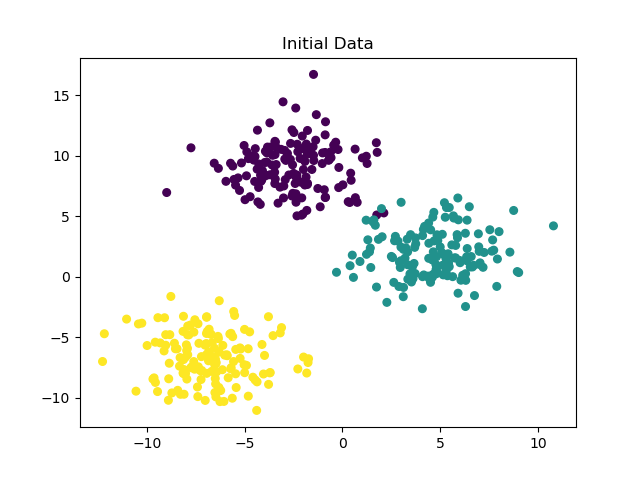
\includegraphics[width=8cm, height=5cm]{pic/original.JPG}
            \end{center}
        \end{figure}
\end{frame}

\begin{frame}{Image Compression}
       \begin{itemize}
           \item 144D to 60D
       \end{itemize}
        \begin{figure}[htpb]
            \begin{center}
                \includegraphics[width=8cm, height=5cm]{pic/60d.JPG}
            \end{center}
        \end{figure}
\end{frame}

\begin{frame}{Image Compression}
       \begin{itemize}
           \item 144D to 16D
       \end{itemize}
        \begin{figure}[htpb]
            \begin{center}
                \includegraphics[width=8cm, height=5cm]{pic/16d.JPG}
            \end{center}
        \end{figure}
\end{frame}


\begin{frame}{Image Compression}
       \begin{itemize}
           \item The 16 most important eigenvectors
       \end{itemize}
        \begin{figure}[htpb]
            \begin{center}
                \includegraphics[width=8cm, height=5cm]{pic/16_most.JPG}
            \end{center}
        \end{figure}
\end{frame}


\begin{frame}{Image Compression}
       \begin{itemize}
           \item 144D to 3D
       \end{itemize}
        \begin{figure}[htpb]
            \begin{center}
                \includegraphics[width=8cm, height=5cm]{pic/3d.JPG}
            \end{center}
        \end{figure}
\end{frame}


\begin{frame}{Image Compression}
       \begin{itemize}
           \item The 3 most important eigenvectors
       \end{itemize}
        \begin{figure}[htpb]
            \begin{center}
                \includegraphics[width=8cm, height=5cm]{pic/3_most.JPG}
            \end{center}
        \end{figure}
\end{frame}


\begin{frame}{Image Compression}
       \begin{itemize}
           \item $L^2$ error and PCA dimensions
       \end{itemize}
        \begin{figure}[htpb]
            \begin{center}
                \includegraphics[width=8cm, height=5cm]{pic/error.JPG}
            \end{center}
        \end{figure}
\end{frame}

\section{Shortcomings and Other Methods}

\begin{frame}{Class Labels}
    \begin{itemize}
        \item PCA doesn’t recognize about class labels.
        \item Alternative solution: Linear Discriminant Analysis (LDA)
        \begin{figure}[htpb]
            \begin{center}
                \includegraphics[width=8cm, height=5cm]{pic/labels.JPG}
            \end{center}
        \end{figure}
    \end{itemize}
\end{frame}


\begin{frame}{Non-Linear}
    \begin{itemize}
        \item PCA cannot capture non-Linear structure.
        \item Alternative solution: Kernel PCA
        \begin{figure}[htpb]
            \begin{center}
                \includegraphics[width=8cm, height=5cm]{pic/nolinear.JPG}
            \end{center}
        \end{figure}
    \end{itemize}
\end{frame}


\begin{frame}{Other Methods}
    \begin{itemize}
        \item \textbf{t-SNE}:
        \begin{itemize}
            \item Non-linear method focusing on preserving local structure.
            \item Often shows well-separated clusters, making it useful for visualization.
            \item Computationally intensive; slower on large datasets.
        \end{itemize}
        \item \textbf{UMAP:}
        \begin{itemize}
            \item Non-linear method that preserves both local and some global structure.
            \item Generally faster than t-SNE and scales better to large datasets.
            \item Can capture more complex structures in the data.
        \end{itemize}
        % \item \textbf{PCA:}
        % \begin{itemize}
        %     \item Linear method; captures the directions of maximum variance.
        %     \item The plot may show overlapping clusters due to its linear nature.
        % \end{itemize}
    \end{itemize}
\end{frame}

\begin{frame}{PCA vs t-SNE vs UMAP}
         \begin{figure}[htpb]
            \begin{center}
                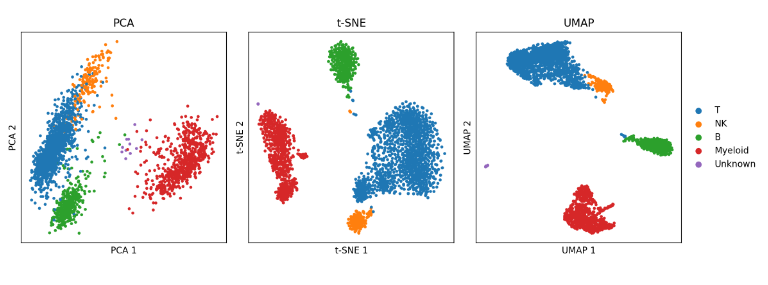
\includegraphics[width=12cm, height=6cm]{pic/tsne_vs_umap_pca.PNG}
                \caption{\href{https://mbernste.github.io/posts/dim_reduc/}{Figure reference}}
            \end{center}
        \end{figure}
\end{frame}

\section{Conclusion}

\begin{frame}{Conclusion}
    \begin{itemize}
        \item PCA 
        \begin{itemize}
            \item Finds orthonormal basis for data
            \item Sorts principal components in order of importance
            \item Discards low significance principal components
        \end{itemize}
        \item Applications
        \begin{itemize}
            \item Get compact description
            \item Remove noise
            \item Improve classification (hopefully)
            \item More efficient use of resources
            \item Statistical
        \end{itemize}
        \item Not magic
        \begin{itemize}
            \item  Doesn’t recognize class labels
            \item Can only capture linear variation
        \end{itemize}
    \end{itemize}
\end{frame}

\section{References}

\begin{frame}{Contributions}
    \begin{itemize}
    \itemsep1em
    \justifying
        \item \textbf{This slide has been prepared thanks to:}
    \begin{itemize}
        \itemsep1em
        \item \href{https://github.com/MohammadMow/}{Mohammad Mowlavi}
    \end{itemize}
    \end{itemize}
\end{frame}

\begin{frame}[allowframebreaks]
    \bibliography{ref}
    \bibliographystyle{ieeetr}
    \nocite{*}
\end{frame}

\end{document}